\chapter{n-3 Polyunsaturated Fatty Acid Rich Diet in Schizophrenia}
\label{omegaProject}
\section{Introduction}
\glsreset{mia}
\glsreset{pufa}
\glsreset{polyic}
\glsreset{gd}
In the previous chapter, we have found that the \gls{SNP} heritability of \glng{scz} was much smaller than expected, accounting for only 20\% of the variance in \glng{scz}.
This suggest that other factors such as rare variants and epigenetic factors might have contributed to the heritability of \glng{scz}.
Another possibility will be the gene environmental interaction ($G\times E$).

Previous studies have suggested there might be interaction between prenatal infection and genetic variations in the development of \glng{scz} \citep{Tienari2004,Clarke2009}.
Evidences now suggest that the effect of prenatal infection was mainly mediated by maternal immune response instead of the specific infection \citep{Brown2010} therefore it is likely that the perturbation induced by \gls{mia} are interacting with genetic variations in the development of \glng{scz}.
With the development of \gls{ldsc}, we may now perform the partitioning of \gls{SNP} heritability using summary statistics from \gls{GWAS}. 
This allow one to investigate whether if a particular functional pathway perturbed by early \gls{mia} contributes disproportionately to the heritability of \glng{scz}.

On the other hand, one of the main goal in \glng{scz} research is to identify effective treatments for \glng{scz} such that the quality of life of schizophrenic patients can be improved. 
Based on the \gls{mia} model, one possible candidate might be the n-3 \gls{pufa} rich diet. 
It has been suggested that n-3 \gls{pufa} can inhibits the production of \gls{il6} \citep{Trebble2003}, which is a major mediator in \gls{mia} \citep{Smith2007}.
Moreover, n-3 \gls{pufa} such as docosahexaenoic acid (DHA) plays a critical role in the development of central nervous system \citep{Clandinin1999,Kitajka2002} and it has robust anti-inflammatory properties \citep{Trebble2003}.
Therefore it is possible that a n-3 \gls{pufa} rich diet can help to alleviate the symptoms of \glng{scz}.
Indeed, previous study from our lab suggested that an n-3 \gls{pufa} rich diet can help to reduce the schizophrenia-like phenotype in mice exposed to early \gls{mia} insults \citep{Li2015}.

% Cerebellum
Herein, we introduce a hypothesis generation study aiming to investigate the gene expression changes induced by early \gls{mia} exposure in the brain of the adult offspring and also expression changes induced by n-3 \gls{pufa} rich diet using RNA Sequencing.
We would also like to investigate whether if functional pathways perturbed by \gls{mia} or changed by diet contributes more to the heritability of \glng{scz} using \gls{ldsc}.

In this study we selected the cerebellum as the target tissue for our experiment. 
Although hippocampus \citep{Velakoulis2006,Nugent2007} and prefrontal cortex \citep{Knable1997,Perlstein2001} are the two most studied region in \glng{scz}, the cerebellum has also been reported to be related to \glng{scz} \citep{Yeganeh-Doost2011,Andreasen2008}.
Moreover, the cerebellum plays a central role in the cortico-cerebellar-thalamic-cortical neuronal circuit which is important to \glng{scz}.
\Gls{pet} studies have shown that a dysfunction in this circuit can contribute to ``cognitive dysmetria'', e.g. impaired cognition and other symptoms of \glng{scz} \citep{Yeganeh-Doost2011}.
Altogether, this makes the cerebellum an interesting target to investigate.

The work in this chapter were done in collaboration with my colleagues who have kindly provide their support and knowledges to make this piece of work possible.
Dr Li Qi and Dr Basil Paul were responsible for generating the animal model and providing the sample for our study;
Dr Li Qi and Dr Desmond Campbell helped with the experimental design;
Vicki Lin has helped with the RNA extraction; 
Tikky Leung for her high quality sequencing service;
Nick Lin for his help in tackling problems encountered during sequencing quality control; 
Dr Johnny Kwan, Dr Desmond Campbell, Dr Timothy Mak and Professor Sham for their guidance in the statistical analysis.

\section{Methodology}
\subsection{Sample Preparation}
Female and male C57BL6/N mice were bred and mated by The University of Hong Kong, Laboratory Animal Unit. 
Timed-pregnant mice were held in a normal light–dark cycle (light on at 0700 hours), and temperature and humidity-controlled animal vivarium. 
All animal procedures were approved by the Committee on the Use of Live Animals in Teaching and Research (CULATR) at The University of Hong Kong.

The \gls{mia} model was generated following procedures previously reported \citep{Li2009c}. 
A dose of 5mg kg$^{-1}$ \gls{polyic} in an injection volume 5ml kg$^{-1}$, prepared on the day of injection was administered to pregnant mice on \gls{gd} 9 via the tail vein under mild physical constraint. 
Control animals received an injection of 5ml kg$^{-1}$ 0.9\% saline. 
The animals were returned to the home cage after the injection and were not disturbed, except for weekly cage cleaning.
The resulting offspring were weaned and sexed at postnatal day 21. 
The pups were weighed and littermates of the same sex were caged separately, with three to four animal per cage.
Half of the animal were fed on diets enriched with n-3 \glspl{pufa} and half were fed a standard  lab diet until the end of the study.
The latter `n-6 \gls{pufa}' control diet had the same calorific value and total fat content as the n-3 \gls{pufa} diet. 
The diets were custom prepared and supplied by Harlan Laboratories (Madison, WI, USA). 
The n-6 and n-3 \gls{pufa} were derived from corn oil or menhaden fish oil, respectively. 
The n-6 \gls{pufa} control diet, was based on the standard AIN-93G rodent laboratory diet \citep{Reeves1993}, and contained 65 g kg$^{-1}$ corn oil and 5 g kg$^{-1}$ fish oil with an approximate (n6)/(n3) ratio of 13:1. 
The n-3 \gls{pufa} diet contained 35 g kg$^{-1}$ corn oil and 35 g kg$^{-1}$ fish oil with an approximate (n6)/(n3) ratio of 1:1 \citep{Olivo2005}.
To avoid being confounded by sex difference, we only use the male offspring for our analysis.
The male offspring were sacrificed by cervical dislocation on postnatal week 12, which roughly correspond to adulthood in human, and the cerebellum was extracted and stored in -80$^{\circ}$C until RNA extraction.

\subsection{RNA Extraction, Quality Control and Sequencing}
Total RNA was extracted from each cerebellum tissue using RNeasy midi kit (Qiagen) following the manufacturer's instructions.
RNA quality was assayed using the Agilent 2100 Bioanalyzer and RNA was quantified using Qubit 1.0 Flurometer.
Samples with \gls{rin} $<7$ were not included in our study as the RNA are most likely degraded.
As a hypothesis generation study, we select a minimum of 3 samples per group and each samples must come from a different litter to control for littering effect.
The RNA Sequencing library was performed at the Centre for Genomic Sciences, the University of Hong Kong, using the KAPA Stranded mRNA-Seq Kit. 
All samples were sequenced using Illumina HiSeq 1500 at 2 lanes (2$\times$101 \gls{bp} paired end reads).
We distribute the samples such that each lane contain roughly the same amount of samples from different conditions.
\begin{table}
	\centering
	\begin{tabular}{rrrrrrr}
		\toprule
		SampleID & Litter & Diet & Condition & Lane & Batch & Rin\\
		\midrule
		B1&	3&	O3&	POL&	1&	B&	7.7\\
		B2&	6&	O3&	POL&	2&	B&	7.7\\
		F1&	4&	O3&	POL&	1&	F&	7.6\\
		F4&	1&	O3&	SAL&	2&	F&	8.1\\
		B4&	5&	O3&	SAL&	1&	B&	7.8\\
		B5&	14&	O3&	SAL&	2&	B&	7.7\\
		F2&	2&	O6&	POL&	1&	F&	7.5\\
		E3&	11&	O6&	POL&	2&	E&	7.8\\
		C2&	7&	O6&	POL&	2&	C&	7.9\\
		B6&	13&	O6&	SAL&	2&	B&	7.4\\
		E6&	14&	O6&	SAL&	1&	E&	8\\
		C6&	1&	O6&	SAL&	1&	C&	7.8\\
		\bottomrule
	\end{tabular}
	\caption[Sample Information]{
		Sample information.
		O3 = n-3 \gls{pufa} diet; O6 = n-6 \gls{pufa} diet; POL = \gls{polyic} exposed; SAL = Saline exposed.
		We have tried to separate the samples into different lane and batch to control for the lane and batch effect. 
		Samples from different litters were also used with the exception of F4 and C6 which came from the same litter but were given a different diet.
		\label{tab:sampleInfo}
	}
\end{table}
\subsection{Sequencing Quality Control}
\Gls{qc} of the RNA Sequencing read data were rather standardized where FastQC \citep{Andrews2010} is the most widely adopted tools.
It can generate the required per base \gls{qc} and provide a general picture of how well the sequencing were done.

From the FastQC report, it was noted that some adapter sequences remained in the final sequence, by using trim\_glore, a wrapper for cutadapt (version 1.9.1) \citep{Martin2011}, we trim the adapter sequences from the sequence reads and only retain reads that were at least 75 \gls{bp} long for subsequent alignment. 

\subsection{Alignment}
In a recent review by \citet{Engstrom2013}, it was demonstrated that STAR \citep{Dobin2013} has the best performance of all the aligners investigated taking into account of accuracy and speed.
Thus STAR aligner was used in our study.
The RNA Sequencing reads were mapped to the \textit{Mus musculus} reference genome (mm10, Ensembl GRCm38.82) using the STAR aligner (version 2.5.0a) \citep{Dobin2013}.
And the quantification of the gene expression levels were conducted using featureCounts (version 1.5.0) \citep{Liao2014}.

\subsection{Differential Expression Analysis}
There are many statistical tools available for the differential gene expression analysis.
Based on the review of \citet{Seyednasrollah2015}, it was suggested that DESeq2 and limma are the most robust statistical packages for analyzing RNA Sequencing data. 
As the authors of DESeq2 are very active in providing supports for the package, we selected DESeq2 (version 2.1.4.5) \citep{Love2014} as the statistic package for the differential gene expression analysis.

Perhaps one of the most controversial study in RNA Sequencing was the mouse ENCODE paper by \citet{Yue2014} where \citet{Gilad2015} demonstrated that most of the findings from \citet{Yue2014} was confounded by lane and batch effect.
This highlights the importance of lane and batch effect in the design of RNA Sequencing.
To avoid batch and lane effect, the whole sampling collection procedure and sequencing was performed in a way where we minimize the batch and lane difference between conditions (\cref{tab:sampleInfo}). 
However, because of the sample quality differs across different batches, we were unable to fully balance out the batch effect. 
Therefore, in our analysis, we must control for the batch effect.

In our study, we were interested in the following comparisons:
\begin{enumerate}
	\item Saline exposed samples with n-3 \gls{pufa} rich diet vs Saline exposed samples with n-6 \gls{pufa} rich diet 
	\item PolyI:C exposed samples with n-3 \gls{pufa} rich diet vs PolyI:C exposed samples with n-6 \gls{pufa} rich diet 
	\item Saline exposed samples with n-6 \gls{pufa} rich diet vs PolyI:C exposed samples with n-6 \gls{pufa} rich diet 
\end{enumerate}
To obtain the desire comparison, and also control for batch effect, we used $\sim Batch+Condition+Diet+Condition:Diet$ as our model of statistical analysis where Condition is the \gls{mia} exposure status.
We did not incorporate the \gls{rin} into our statistic model because it was advised against by the author.

We would also like to see if the batch effect can leads to false positive results.
Therefore we performed the \gls{lrt} to investigate the effect of batch on our result.
The \gls{lrt} examines two models for the counts, a full model with a certain number of terms and a reduced model, in which some of the terms of the full model are removed. 
The test determines if the increased likelihood of the data using the extra terms in the full model is more than expected if those extra terms are truly zero.
Thus we compared the full model $\sim Batch+Condition+Diet+Condition:Diet$ with $\sim Condition+Diet+Condition:Diet$ to understand the effect of batch on our data.

In our analysis, we removed all genes with base mean count $<$ 10  to reduce the noise associated with low expression and the Benjamini and Hochberg method were then used to correct for multiple testing.

\subsection{Functional Annotation}
\label{sec:function}
One of the most important aim of the current study is to investigate whether if functional pathways perturbed by \gls{mia} or affected by diet contribute to larger amount of \gls{SNP} heritability.
It is therefore important to perform functional annotation of the \glspl{deg} in order to identify pathways that were affected (e.g. enriched by the \glspl{deg}).

Because of the limited number of \gls{deg} identified, we performed the Wilcoxon Rank Sum test to test whether if genes within the pathway are more significant the genes outside pathway.
The canonical pathways annotations obtained from the \gls{msigdb} (v5.0 updated April 2015) \citep{Subramanian2005} were used for our analysis.
To avoid testing overly narrow or broad functional pathways, pathways with more than 300 genes or less than 10 genes were removed from our analysis. 
Pathways with adjusted p-value $<0.05$ (using Benjamini and Hochberg adjustment) were considered as significant.

\subsection{Partitioning of Heritability}
We then tried to perform partitioning of heritability using the significant pathways as our annotation.
One problem with the pathways is that they can overlap with each other and can even be a sub-pathway of another pathway.
We therefore calculated the Jaccard distance between each pathways:
\begin{equation}
\text{Jaccard distance} = \frac{Overlapped\ Genes}{Total\ Number\ of\ Unique\ Genes}
\end{equation}
For pathways with a Jaccard distance greater than 0.2, we removed the smaller pathway, thus reducing the number of pathways in the analysis.
Two ``super pathways'' were also generated which included all the genes in the pathways perturbed in \gls{mia} or genes in pathways affected by diet. 

\glspl{SNP} from the 1000 genome was first associated with genes using SnpEFF \citep{Cingolani2012} with the GRCh37.75 annotation, where \glspl{SNP} within $\pm5$\gls{kb} region of a gene was considered to be associated.
The annotation file required by \gls{ldsc} was then generated by identifying \glspl{SNP} participated in the significant pathways from \cref{sec:function}.
If a \gls{SNP} was found to be associated with more than 1 genes, then it was considered to be within all pathways where its associated genes were part of. 

Finally, we performed the partitioning of heritability using \gls{ldsc} \citep{Bulik-Sullivan2015} -{}-annot and -{}-overlap-annot options using 1000\gls{kb} window size and the reference panel generated from \cref{sec:realData}.
We removed the \gls{mhc} region from this analysis.
Pathways with positive proportion of heritability explained and a \gls{fdr} q-value $<0.125$ were considered significant.
We considered the ``super pathways'' as a super test which included all the pathways tested, therefore we did not perform any multiple testing correction on it.

\subsection{Designing the Replication Study}
Another important goal of our current study is to provide information for further replication studies. 
In order to estimate the power and required samples for the replication studies, we performed the power estimation using Scotty \citep{Busby2013}.
We provided the count data from our pilot samples to Scotty to estimate the minimal required samples for our replication study if we would like to detect at least 90\% of the genes that are differentially expressed by a 2$\times$ fold change at p$<0.01$ and that at least 80\% of genes has at least 80\% of the maximum power.

%TODO until here
\section{Results} 
\subsection{Sample Quality}
On average, 87 million reads were generated for each sample of which more than 90\% of the read bases has quality score $>30$.
A quality score at 30 represents the probability of having an incorrect base call is less than 1 in 1,000.
After removing the adapter sequences from the reads, more than 97\% of the reads remains.
Over 90\% of the trimmed reads could be uniquely mapped to the \textit{Mus musculus} reference genome (mm10, Ensembl GRCm38.82) using the STAR aligner (version 2.5.0a) \citep{Dobin2013}.
To obtained the expression count, we used the featureCounts (version 1.5.0) \citep{Liao2014} to generate the count matrix required for downstream analysis.

Next, we were interested in whether if there are any contamination of samples or series confounding effect of bath or lane.
We therefore performed an unsupervised clustering on the sample count data.
It was observed that none of the samples were clustered by lane or batch, suggesting that there were no serious batch or lane effect presented in our samples.
However, one sample from the n3-\gls{polyic} group was found to be substantially different from all other samples (\cref{fig:distMatrix}).
It was unclear whether if the difference was due to sample contaminations (from other source) or was due to sample mis-label.
To avoid problems in down-stream analysis, we excluded this sample from subsequent analyses.
 \begin{figure}
	\centering
	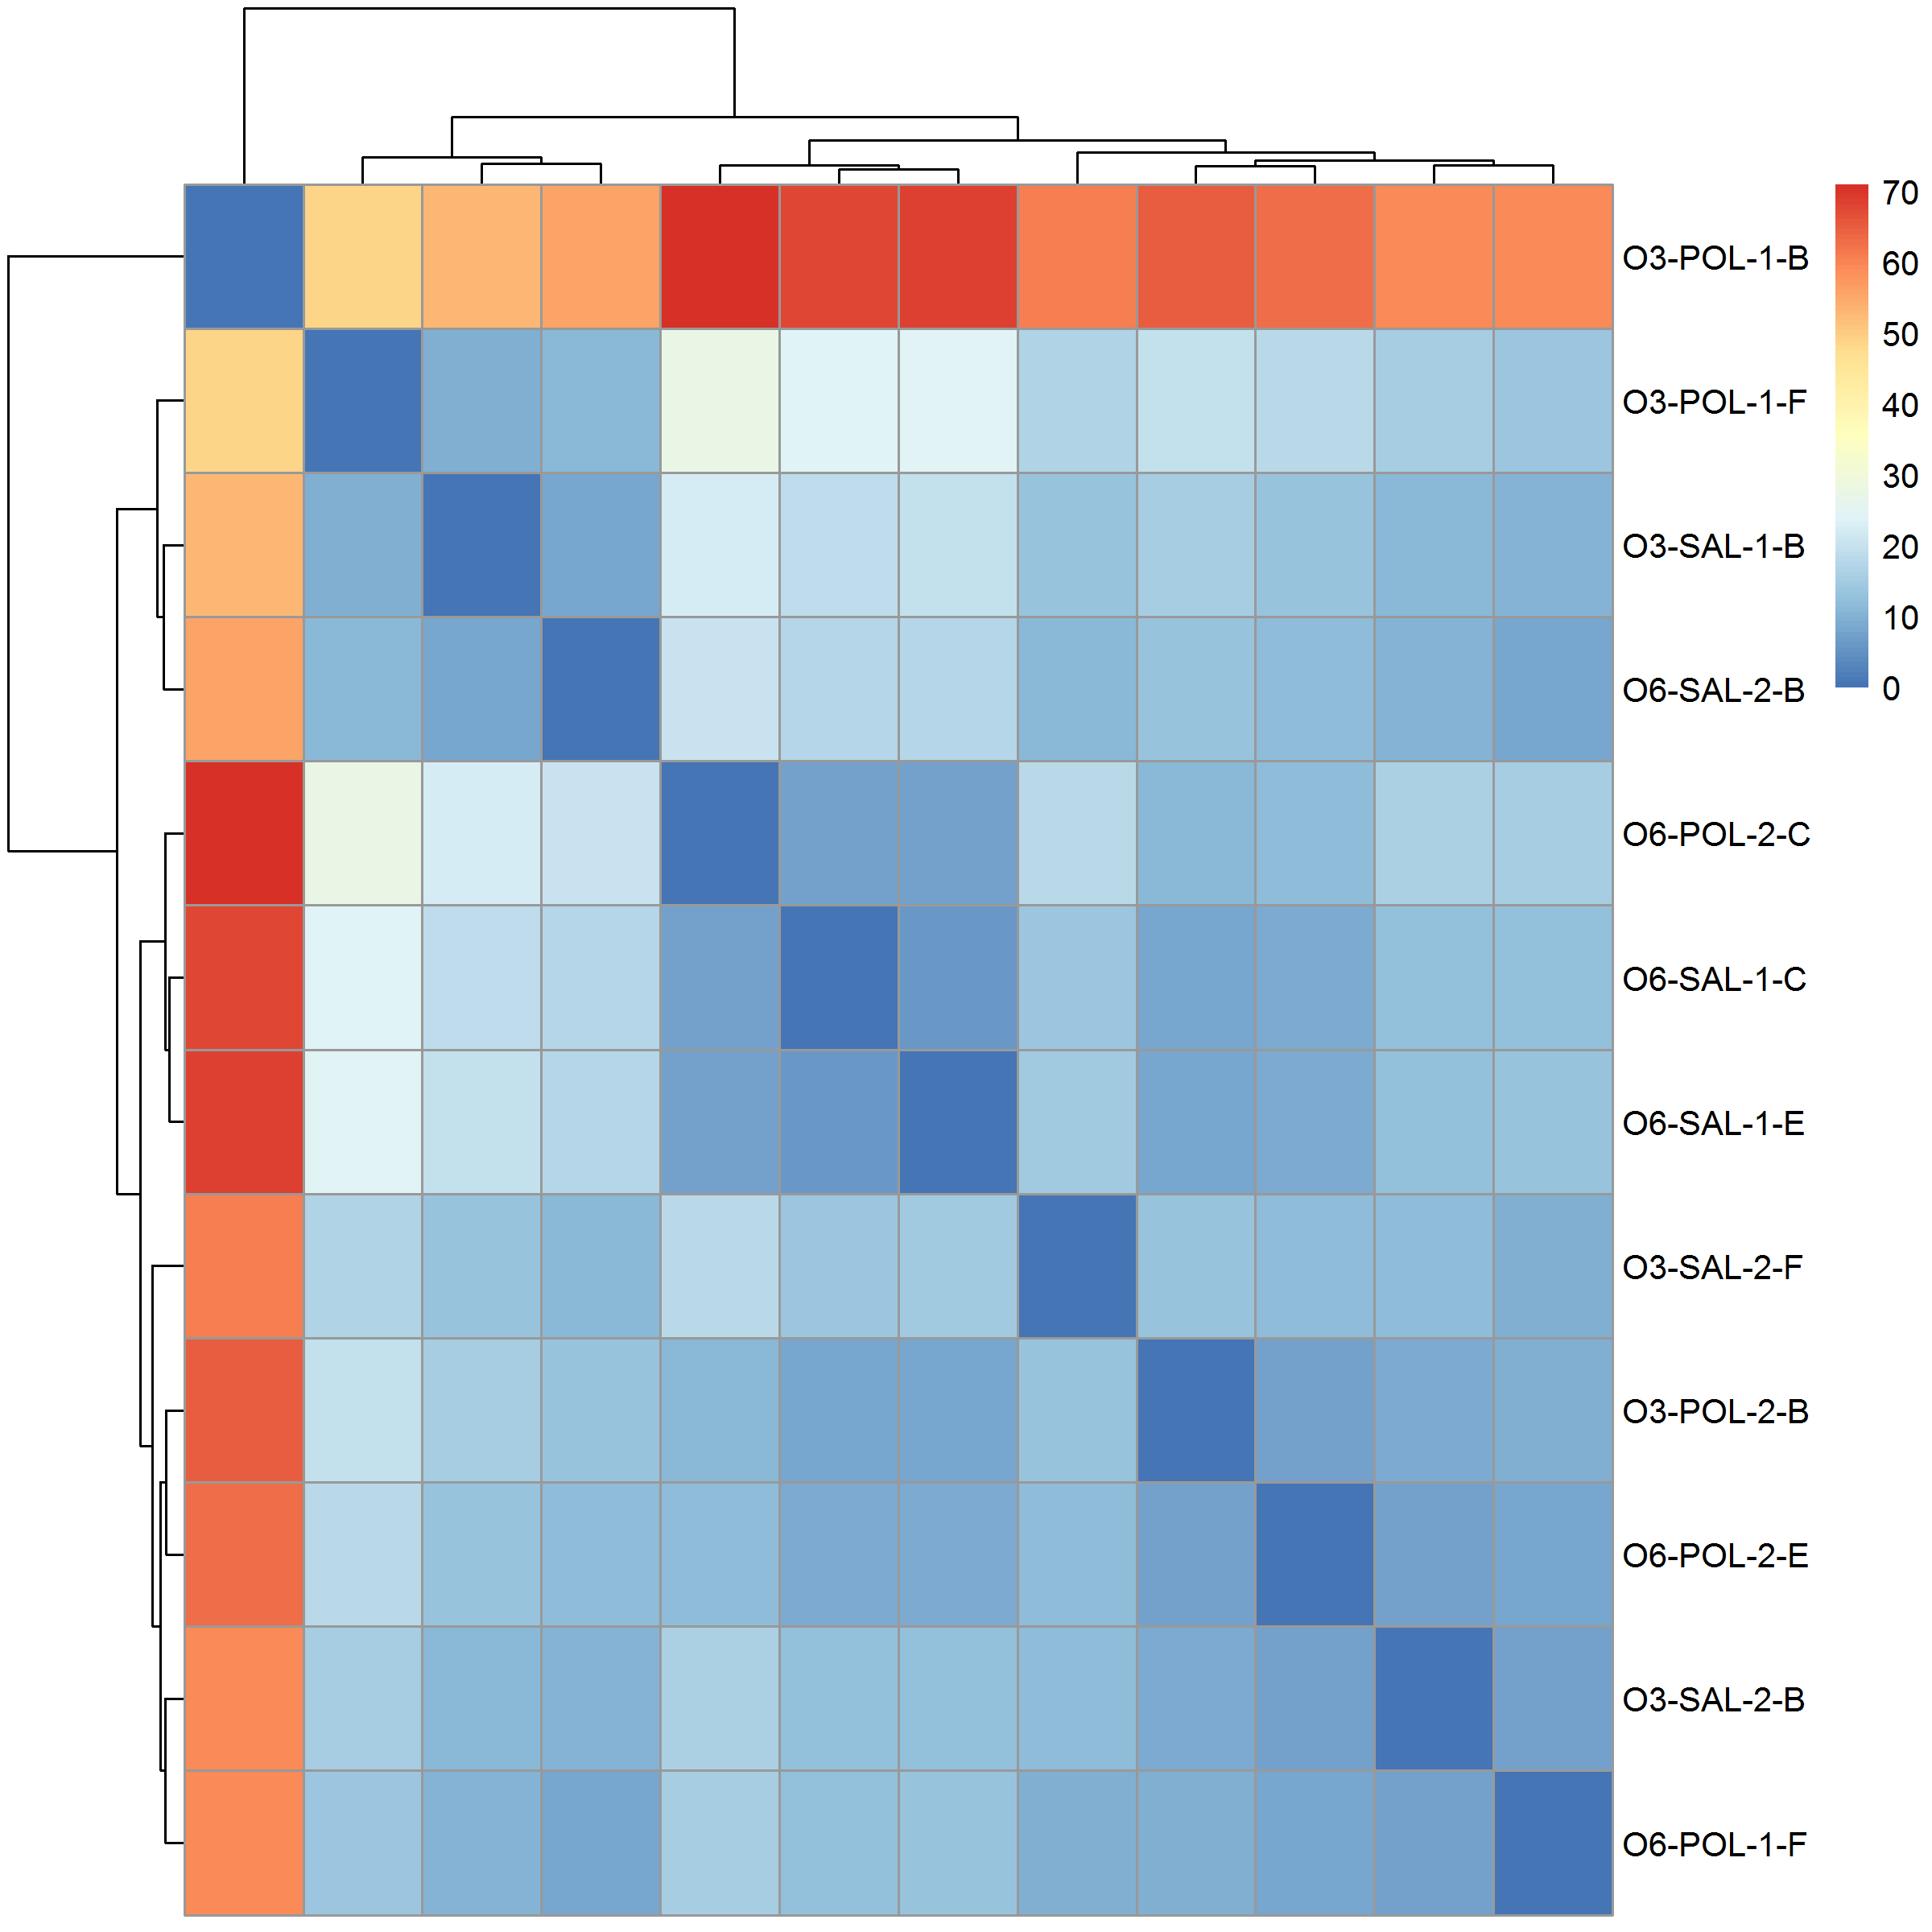
\includegraphics[width=0.7\textwidth]{figure/DistanceMatrix.png}
	\caption[Sample Clustering]{Sample Clustering results.
		It was observed that there was no clear clustering for lane or batch effects.
		However, one sample from the n3-\gls{pufa}-\gls{polyic} group was found to be substantially different from all other samples.
		
		It was unclear whether if the difference was due to sample contaminations or was due to sample mis-label.
		To avoid problems in down-stream analysis, we excluded this sample from subsequent analyses }
	\label{fig:distMatrix}
 \end{figure}
\subsection{Differential Expression Analysis}
\begin{figure}
	\centering
	\subfloat[O6-Saline mice vs O6-PolyI:C mice]{
		\scalebox{.4}{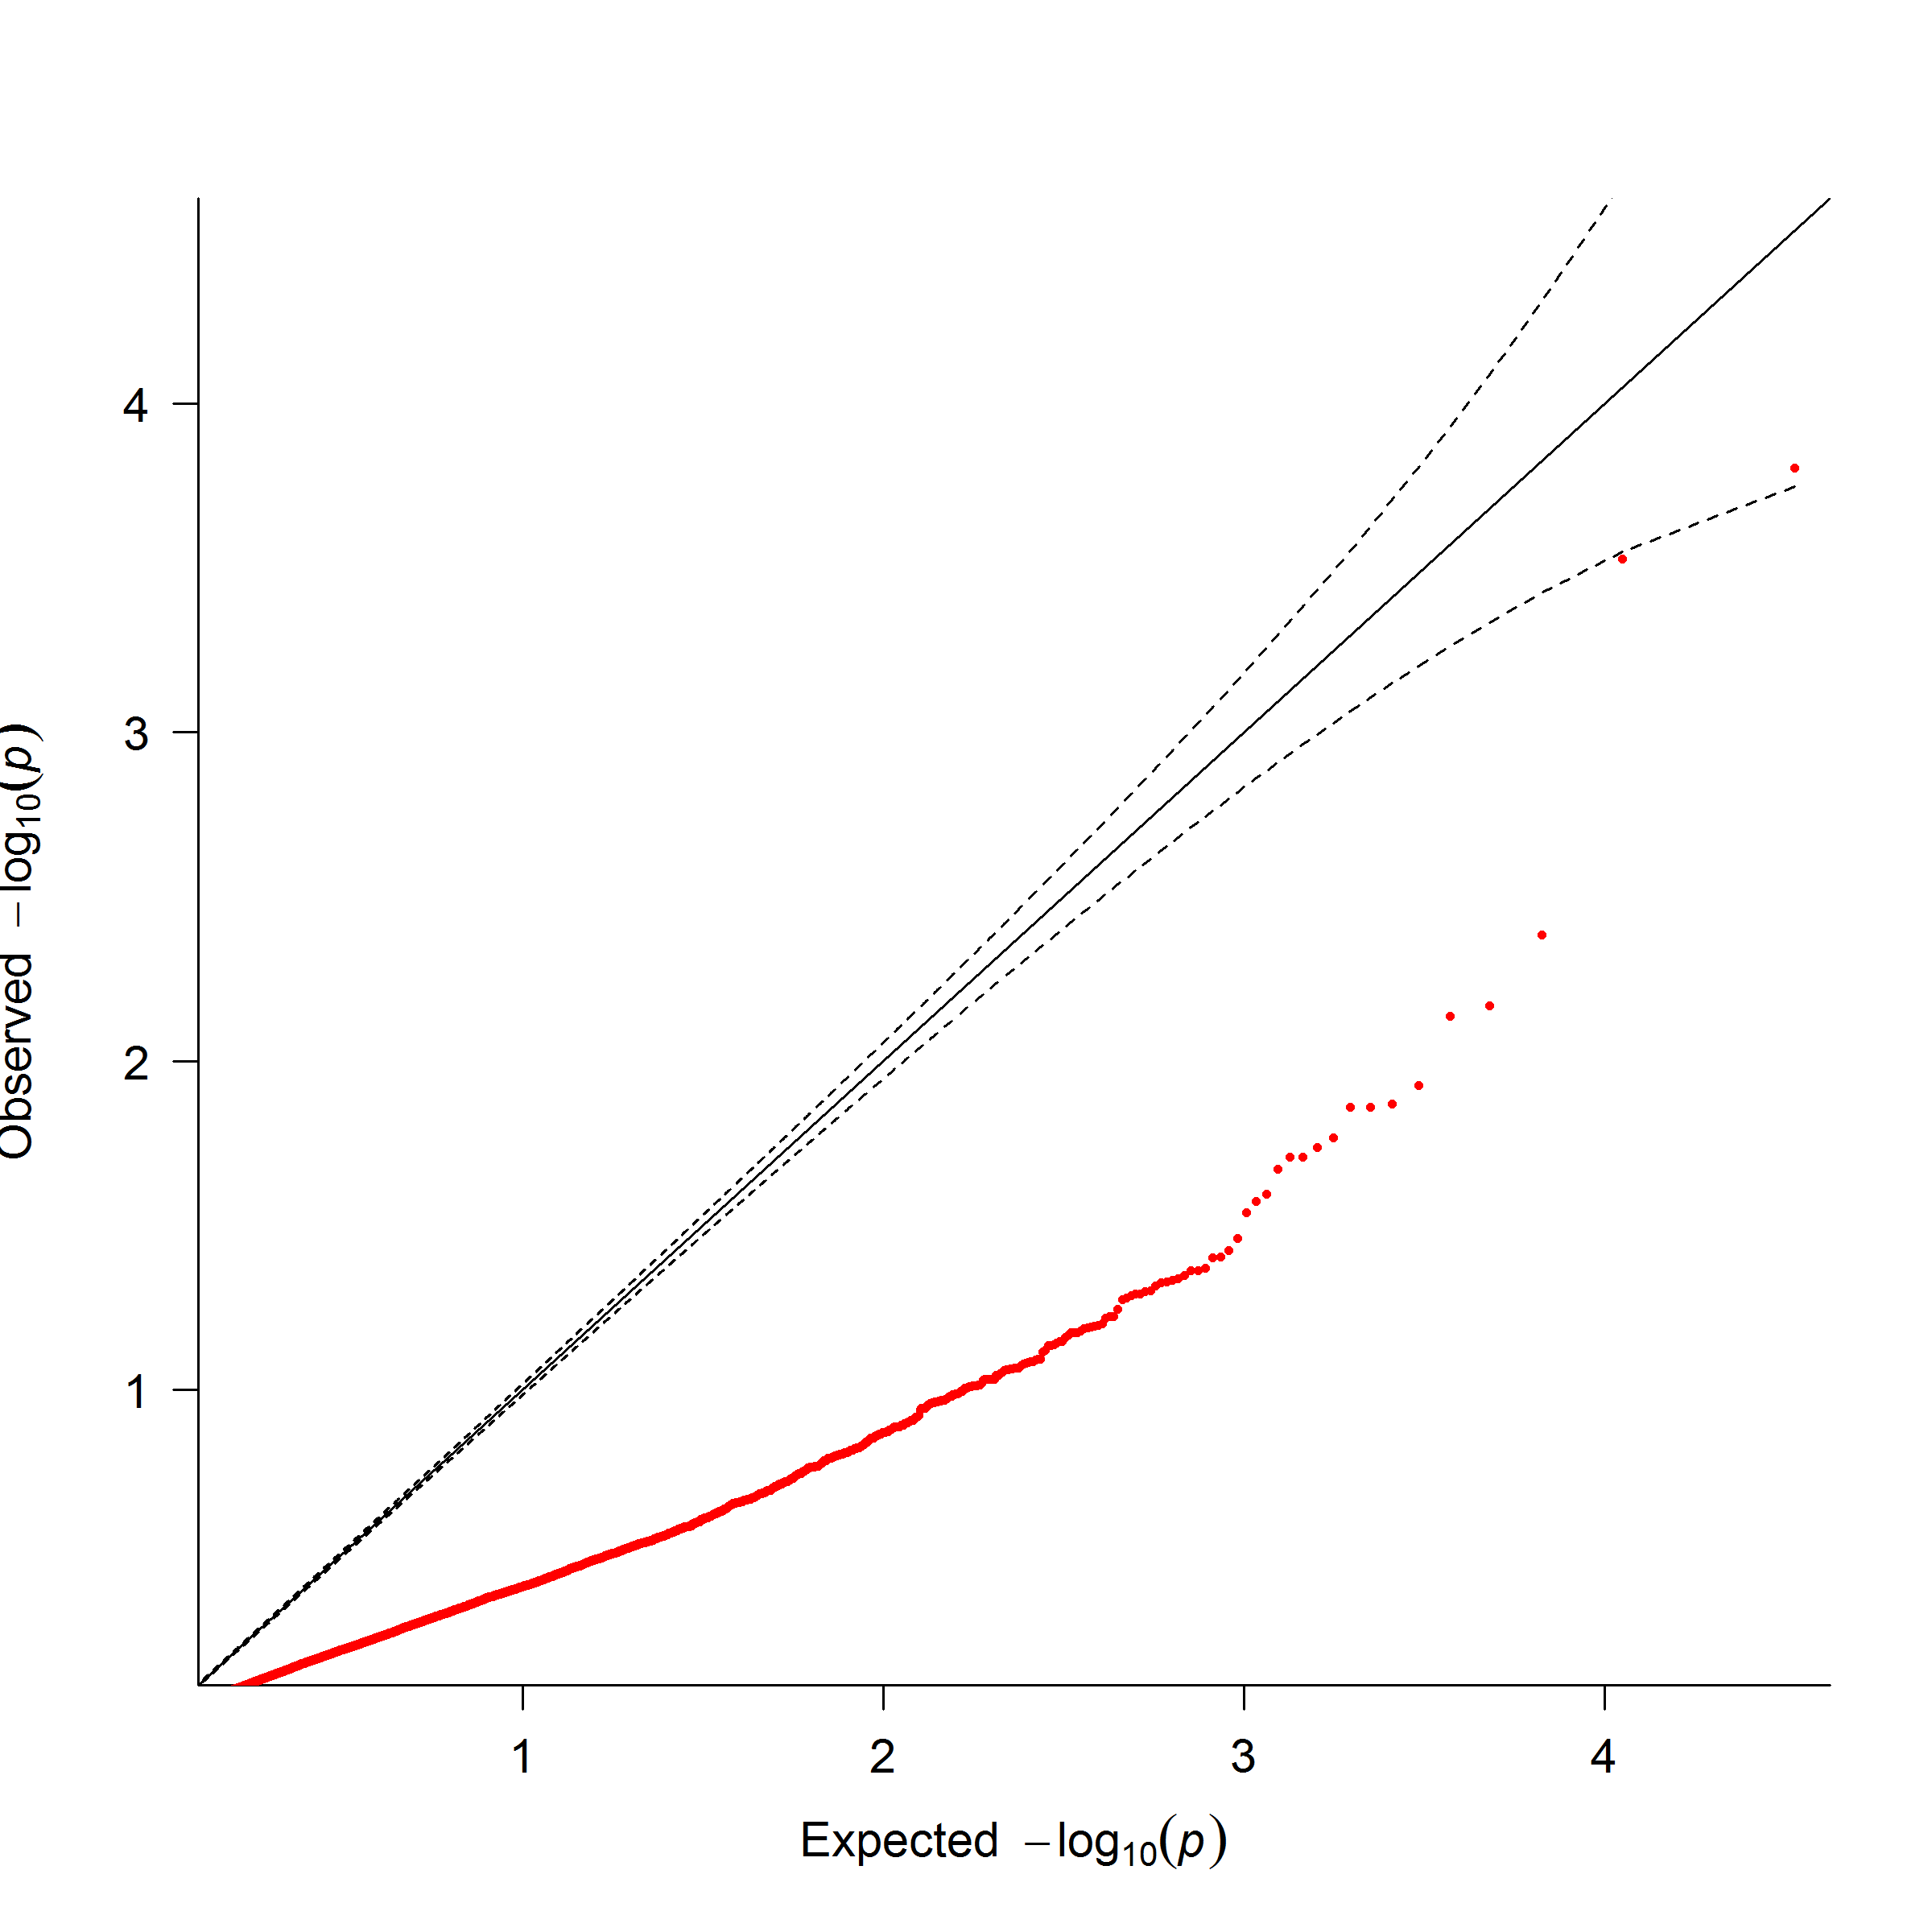
\includegraphics{figure/omega/miaO6_wald_qq.png}}
		\label{fig:miaO6Wald}
	}
	\subfloat[O6-Saline mice vs O3-Saline mice]{
		\scalebox{.4}{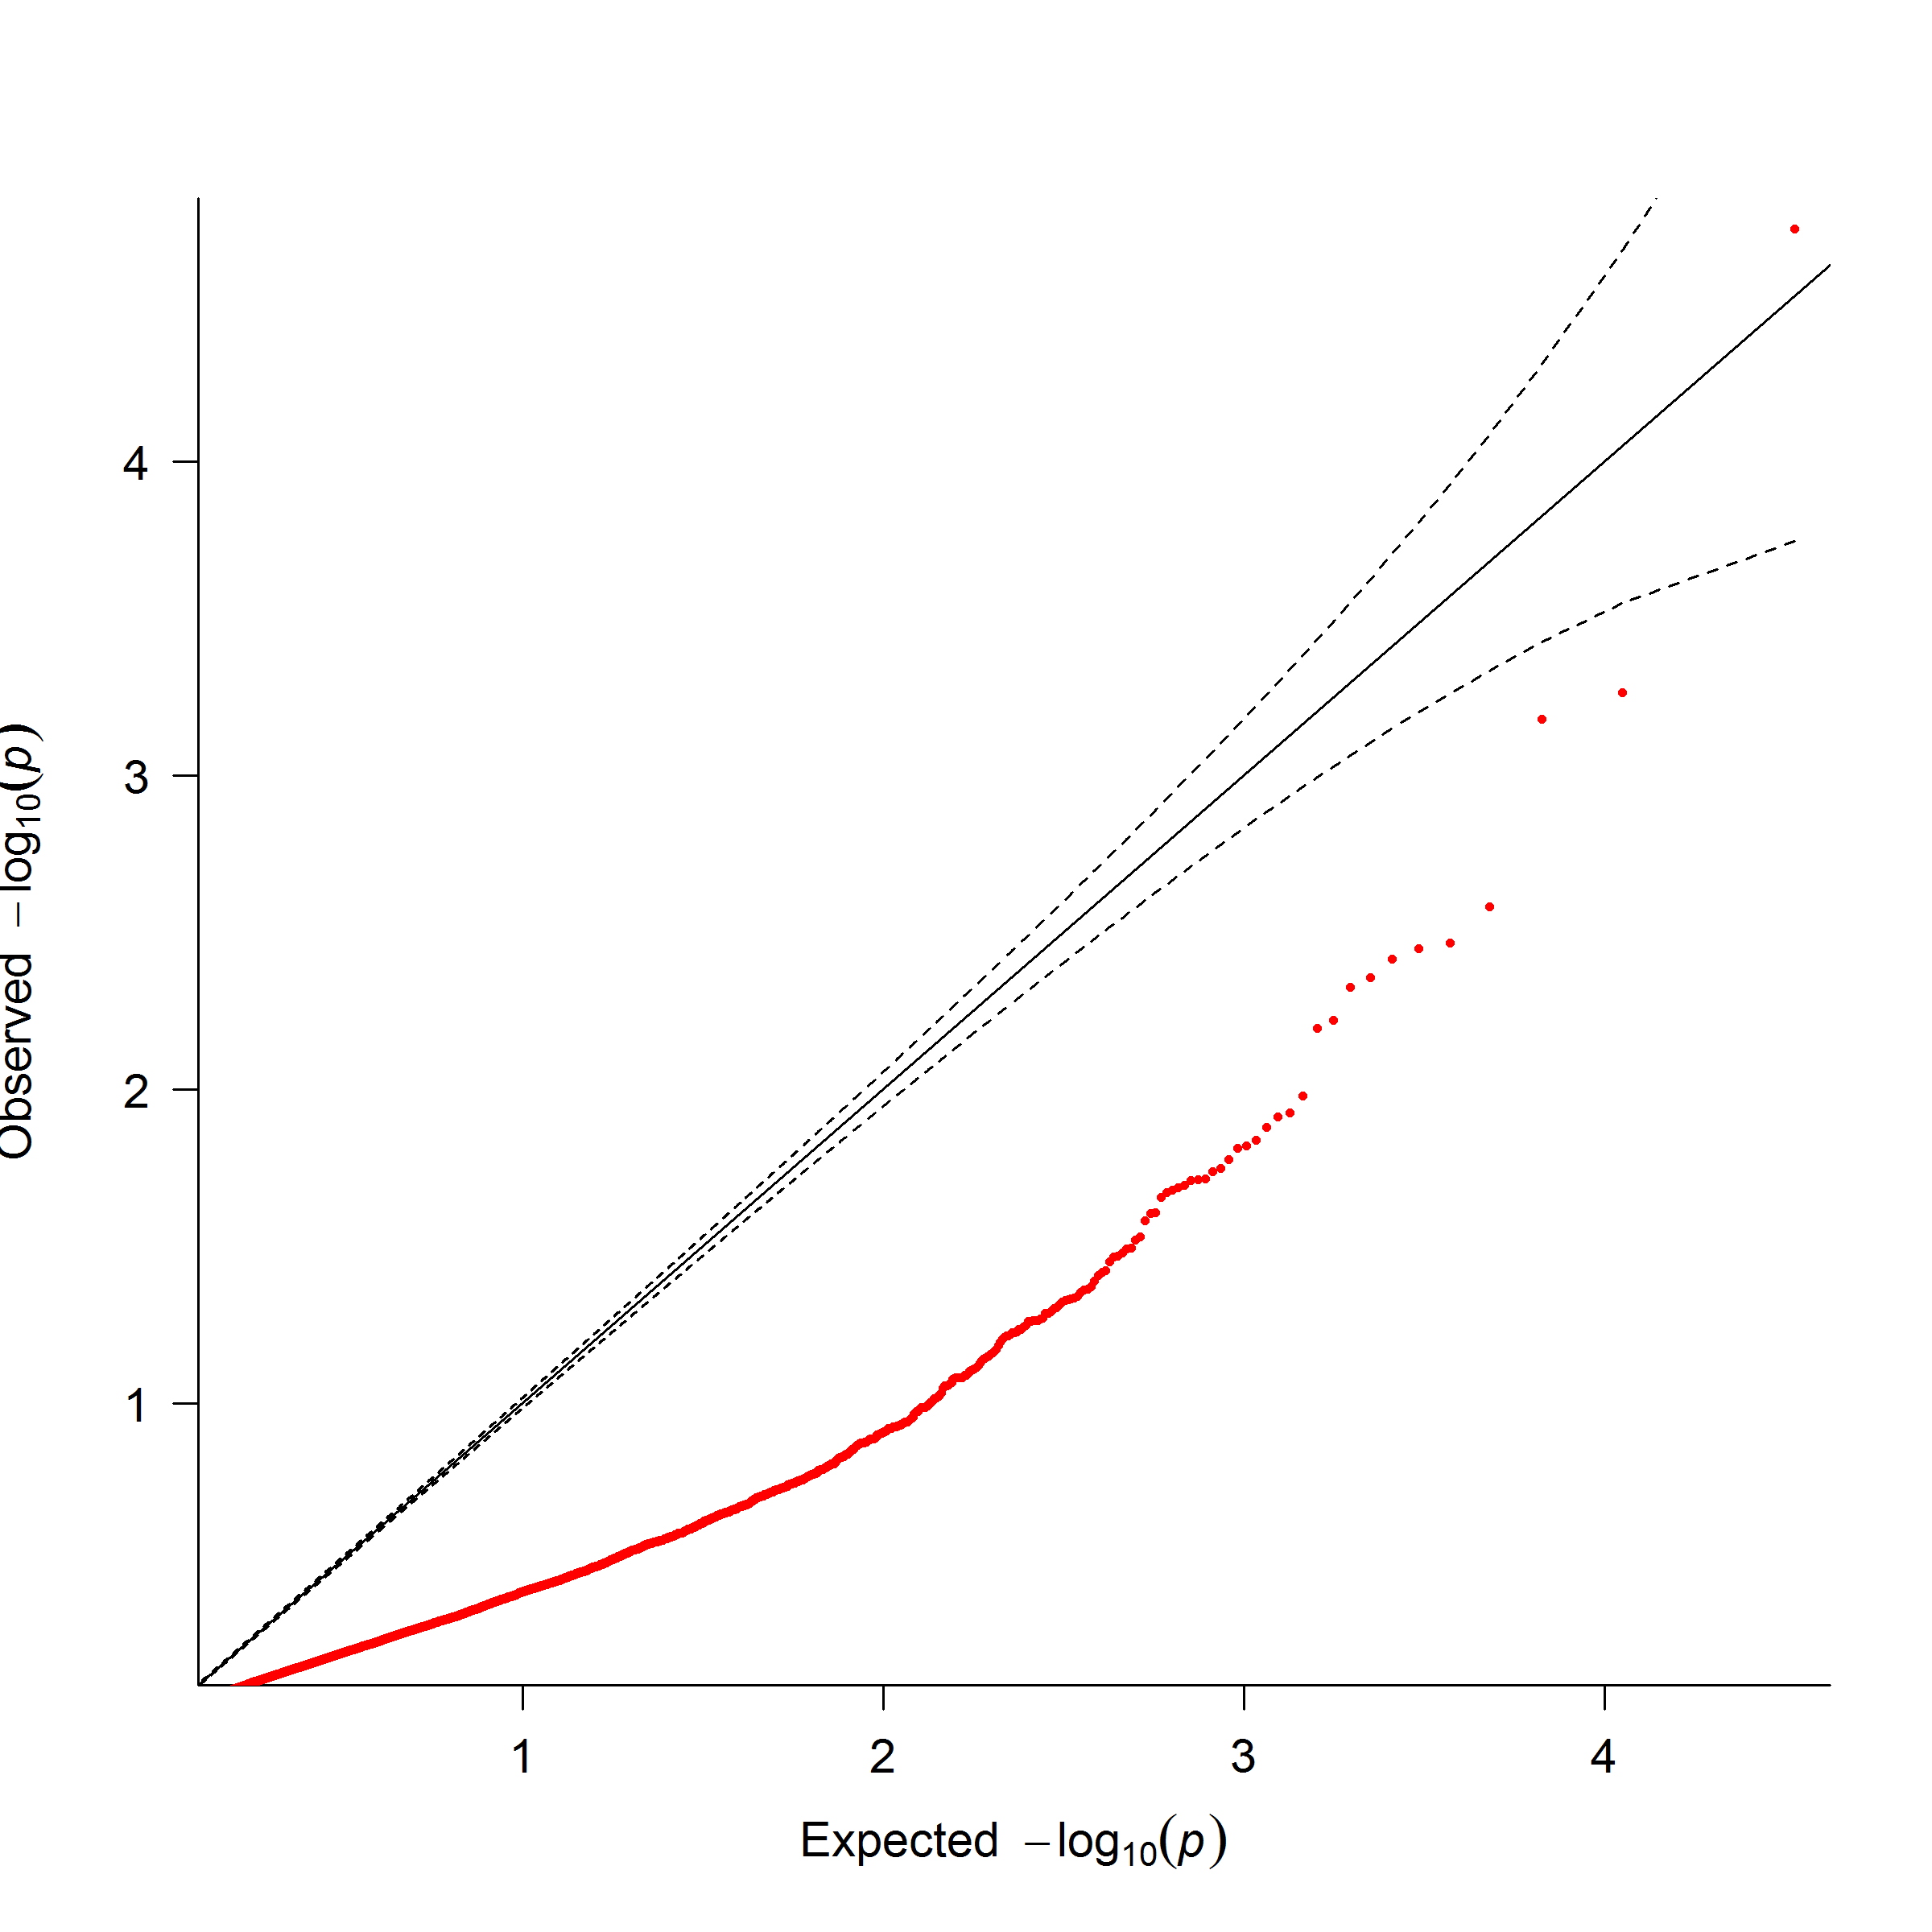
\includegraphics{figure/omega/omegaSAL_wald_qq.png}}
		\label{fig:omegaSALWald}
	}\\
	\subfloat[O6-PolyI:C mice vs O3-PolyI:C mice]{
		\scalebox{.4}{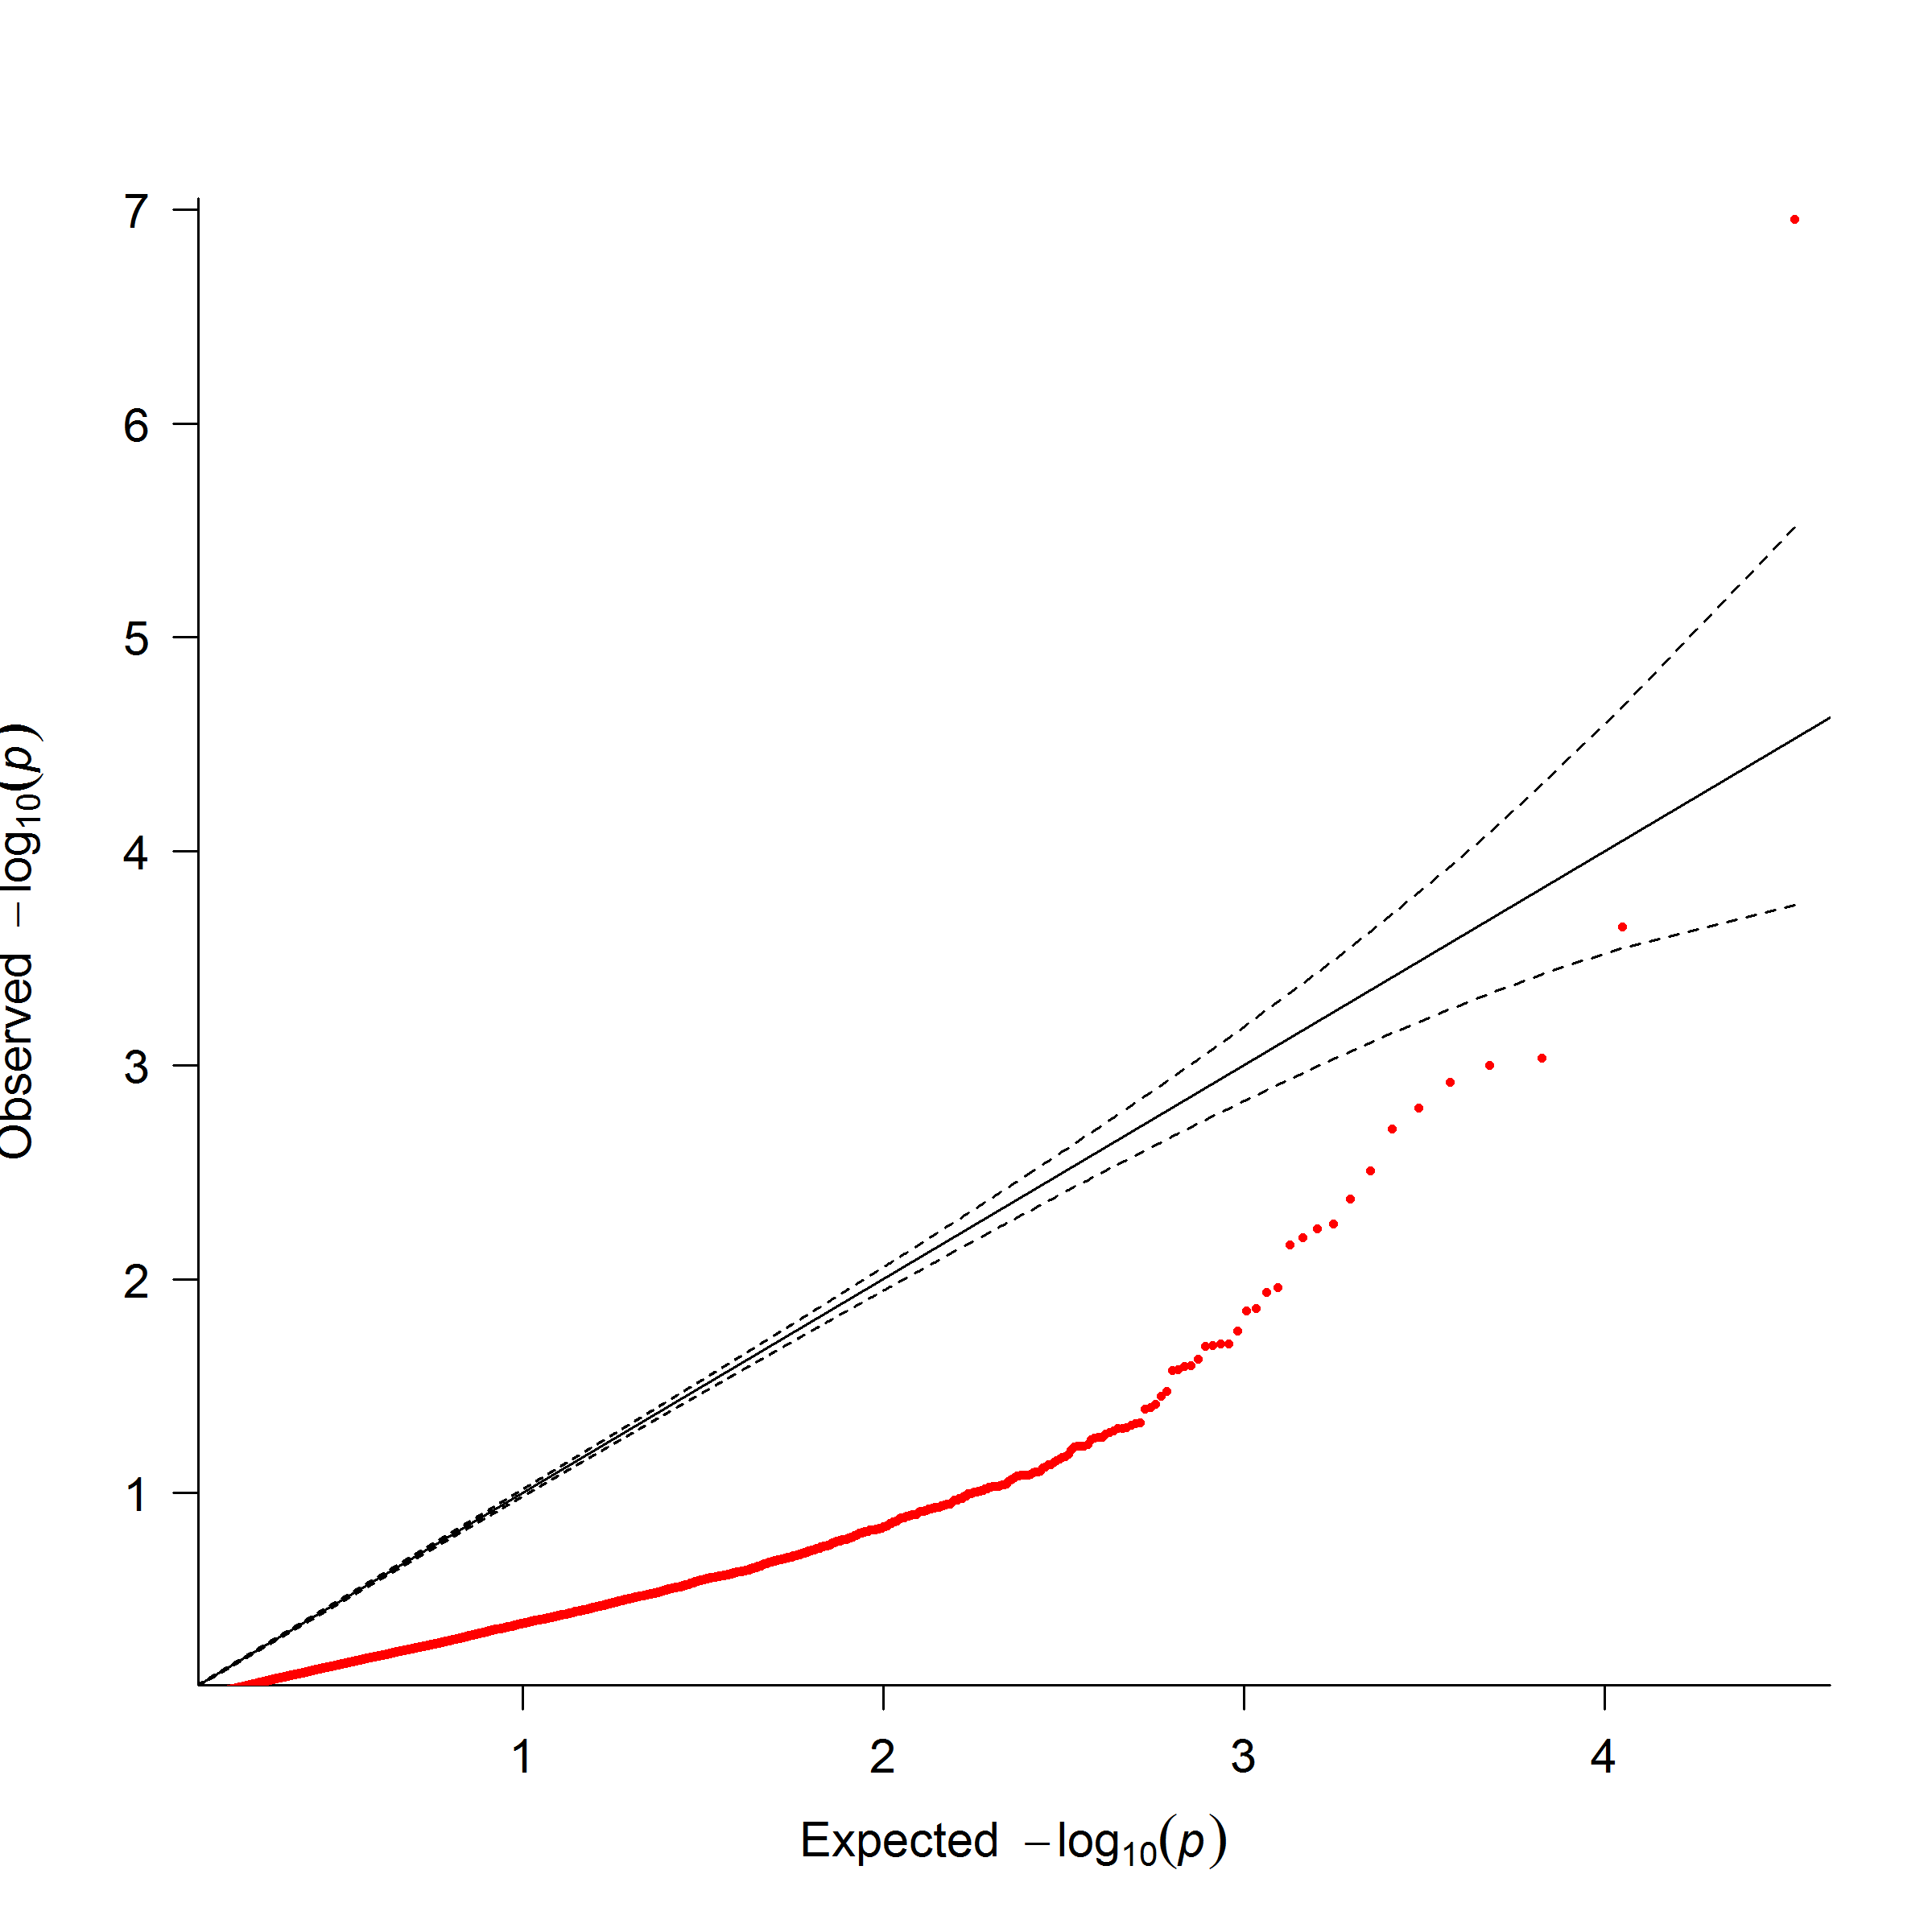
\includegraphics{figure/omega/omegaPOL_wald_qq.png}}
		\label{fig:omegaPOLWald}
	}
	\subfloat[Batch Effect]{
		\scalebox{.35}{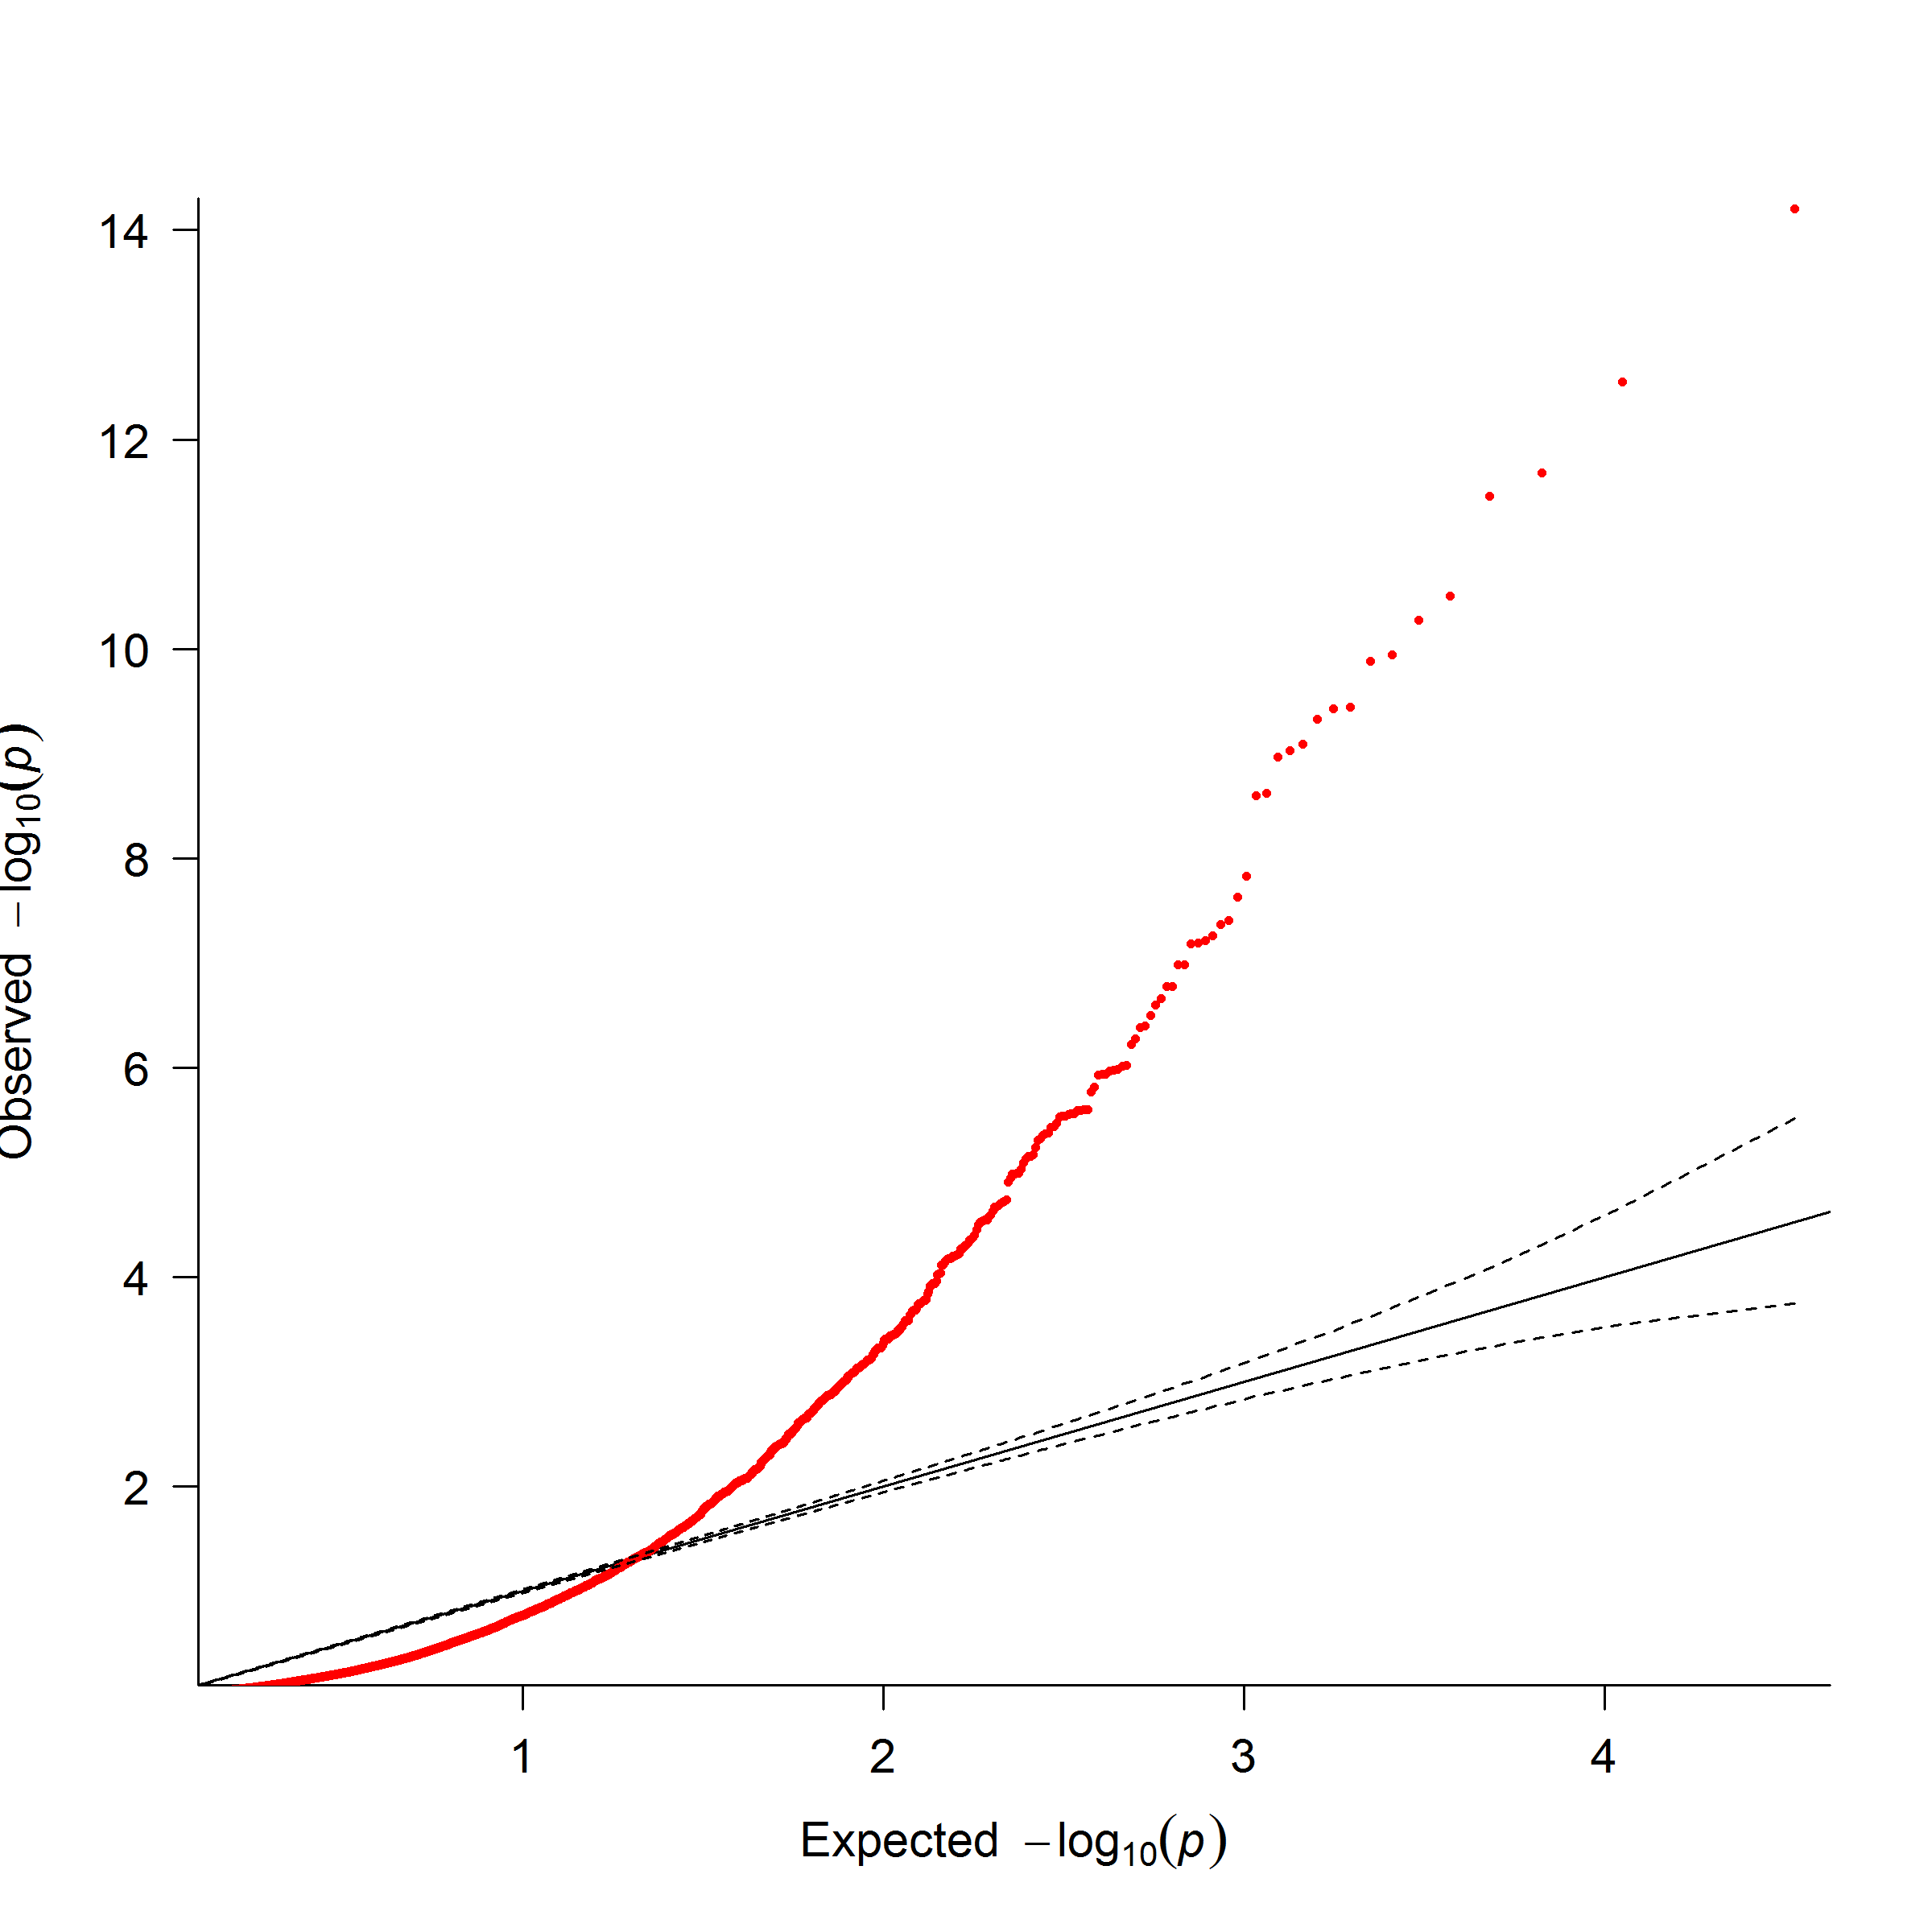
\includegraphics{figure/omega/nobatch_lrt.png}}
		\label{fig:batchLRT}
	}
	\caption[QQ Plot Statistic Results]
	{QQ Plot of statistic results.
		From the \gls{qqplot}, it was observed that most of the observed p-value was less than what would have been expected. 
		This is likely due to the small sample size of our study which leads to an under powered association.
		The only exception was the analysis of batch effect were a large amount of genes were found to be significant. 
		This demonstrate the importance of adjusting for batch effect} 
	\label{fig:waldQQ}
\end{figure}
After excluding the problematic samples, we performed the DESeq2 analysis.
Of the 16,747 genes that passed through quality control, only one gene, \textit{Sgk1} (p-adjusted=0.00186) was found to be significantly differentiated when we examines the effect of n-3 \gls{pufa} rich diet on the gene expression in the cerebellum of \gls{polyic} exposed mice (\cref{fig:omegaPOLWald}).
No gene was found to be significant for the other two comparisons (\cref{fig:miaO6Wald,fig:omegaSALWald}).

We also performed the \gls{lrt} to compare test the effect of batch on our analysis. 
A total of 178 genes were found to be significant differentiated (\cref{fig:batchLRT}), suggesting that the ``Batch'' is indeed an important factor to consider in our analysis.

\subsection{Functional Annotation}
It is common practice to perform functional annotation to the \glspl{deg}. 
However, in most of our analysis, there were either no \gls{deg} or only 1 \gls{deg}, making it difficult to perform functional annotation.
We therefore used the Wilcox rank sum test to analysis whether if a pathway contain genes that are more significant than genes not within the pathway.

None of the pathways were found to be significant when comparing the effect of the n-3 \gls{pufa} rich diet in Saline exposed mice. 
On the contrary, 17 pathways were found significant when comparing the effect of n-3 \gls{pufa} rich diet in \gls{polyic} exposed samples (\cref{tab:o6polyPath}) where 4 pathways were related to growth factors such as \gls{fgf} or \gls{egf} and 4 others were related to kinases such as \gls{pi3k} or \gls{mapk}.

Finally, 12 pathways were found to be significant when comparing Saline and \gls{polyic} exposed mice given the n-6 \gls{pufa} rich diet (\cref{tab:miaPath}) with pathways such as neuroactive ligand-receptor interaction (p-adj = $1.27\times10^{-3}$), calcium signaling pathway (p-adj = $2.79\times10^{-3}$) and genes involved in Neuronal System (p-adj=0.00153) among the significant pathways.

\subsection{Partitioning of Heritability}
Given the significant pathways, we performed the partitioning of heritability using \gls{ldsc} \citep{Bulik-Sullivan2015}.
In total, 14 unique pathways were included in the analysis were 4 of them were found to have non-negative contribution to the heritability of \glng{scz}, including the pathway related to neuronal system, \gls{ecm} glycoprotein, calcium signaling and \gls{mapk} signaling (\cref{tab:partitioning}).
All of these pathways were affected by \gls{mia} and only the \gls{ecm} pathways were also found to be affected by n-3 \gls{pufa} rich diet in \gls{polyic} exposed mice.
Moreover, the ``super pathway'' for \gls{mia} were found to be significant (p-value=0.0402) yet the ``super pathway'' for diet was found to be insignificant (p-value=0.414).

\subsection{Designing the Replication Study}
Other than generation of hypothesis, we would also like to use the current information to help designing subsequent replication studies.
Using Scotty \citep{Busby2013}, given that we would like to detect at least 90\% of the genes that are differentially expressed by a 2$\times$ fold change at p$<0.01$ and that at least 80\% of genes has at least 80\% of the maximum power, we will need at least 10 samples per group in the replication study given the current sequencing depth.

\begin{landscape}
	\begin{table}
		\begin{tabular}{rrrp{10cm}r}
			\toprule
			ID&	Size&	Source&	Description&	Adjusted P-Value\\
			\midrule
			M508&	78&	REACTOME&	Genes involved in Signaling by SCF-KIT&	0.00671\\
			M570&	44&	REACTOME&	Genes involved in PI3K events in ERBB2 signaling&	0.0242\\
			M3008&	196&	NABA&	Genes encoding structural ECM glycoproteins&	0.0309\\
			M1090&	112&	REACTOME&	Genes involved in Signaling by FGFR&	0.0309\\
			M563&	109&	REACTOME&	Genes involved in Signaling by EGFR in Cancer&	0.0309\\
			M17776&	100&	REACTOME&	Genes involved in Downstream signaling of activated FGFR&	0.0309\\
			M1076&	83&	REACTOME&	Genes involved in Amyloids&	0.0309\\
			M850&	56&	REACTOME&	Genes involved in PI-3K cascade&	0.0309\\
			M10450&	38&	REACTOME&	Genes involved in GAB1 signalosome&	0.0309\\
			M16227&	24&	REACTOME&	Genes involved in Cholesterol biosynthesis&	0.0309\\
			M5872&	17&	KEGG&	Steroid biosynthesis&	0.0309\\
			M16334&	10&	BIOCARTA&	Eph Kinases and ephrins support platelet aggregation&	0.0309\\
			M5884&	275&	NABA&	Ensemble of genes encoding core extracellular matrix including ECM glycoproteins, collagens and proteoglycans&	0.0456\\
			M635&	127&	REACTOME&	Genes involved in Signaling by FGFR in disease&	0.0456\\
			M568&	38&	REACTOME&	Genes involved in PI3K events in ERBB4 signaling&	0.0456\\
			M165&	32&	PID&	Syndecan-4-mediated signaling events&	0.0456\\
			M1262&	15&	REACTOME&	Genes involved in GRB2:SOS provides linkage to MAPK signaling for Intergrins&	0.0456\\
			\bottomrule
		\end{tabular}
		\caption[Significant Pathways When Comparing Effect of Diet in PolyI:C Exposed Mouse]{Significant Pathways when comparing effect of diet in \gls{polyic} exposed mice.
			The pathway IDs are the systematic name from \gls{msigdb}.
			Most of the significant pathways were related to the kinase such as PI3K and MAPK or growth factors such as \gls{fgf} and \gls{egf}.
		}
		\label{tab:o6polyPath}
	\end{table}
	
	\begin{table}
		\begin{tabular}{rrrp{10cm}r}
			\toprule
			ID&	Size&	Source&	Description&	Adjusted P-Value\\
			\midrule
			M13380&	272&	KEGG&	Neuroactive ligand-receptor interaction&	$1.27\times10^{-3}$\\
			M2890&	178&	KEGG&	Calcium signaling pathway&	$2.79\times10^{-3}$\\
			M12289&	188&	REACTOME&	Genes involved in Peptide ligand-binding receptors&	0.00118\\
			M5884&	275&	NABA&	Ensemble of genes encoding core extracellular matrix including ECM glycoproteins, collagens and proteoglycans&	0.00119\\
			M735&	279&	REACTOME&	Genes involved in Neuronal System&	0.00153\\
			M15514&	186&	REACTOME&	Genes involved in Transmission across Chemical Synapses&	0.00401\\
			M4904&	121&	REACTOME&	Genes involved in G alpha (s) signalling events&	0.0127\\
			M3008&	196&	NABA&	Genes encoding structural ECM glycoproteins&	0.0131\\
			M752&	137&	REACTOME&	Genes involved in Neurotransmitter Receptor Binding And Downstream Transmission In The Postsynaptic Cell&	0.0131\\
			M10792&	267&	KEGG&	MAPK signaling pathway&	0.0195\\
			M17&	59&	PID&	Notch signaling pathway&	0.0406\\
			M18437&	184&	REACTOME&	Genes involved in G alpha (q) signalling events&	0.0406\\
			\bottomrule
		\end{tabular}
		\caption[Significant Pathways When Comparing Effect of PolyI:C in Mouse Given n-6 \gls{pufa} Rich Diet]{Significant pathways when comparing effect of PolyI:C in mouse given n-6 \gls{pufa} rich diet.
			The pathway IDs are the systematic name from \gls{msigdb}.
			Interestingly, we observed a lot of neural related pathways and even got significant signal in the calcium signaling pathway, which was reported to be associated with \glng{scz} \citep{Purcell2014}. 
		}
		\label{tab:miaPath}
	\end{table}
	
	\begin{table}
		\begin{tabular}{rrrp{9cm}p{1.7cm}p{1.5cm}p{1.7cm}}
			\toprule
			ID& Size&	Source&	Description&	Proportion of $h^2$&	SE&	Enrichment Q-Value\\
			\midrule
			M735&	279&	REACTOME&	Genes involved in Neuronal System&	0.0287&	0.00627&	0.0456\\
			M5884&	275&	NABA&	Ensemble of genes encoding core extracellular matrix including ECM glycoproteins, collagens and proteoglycans&	0.00363&	0.00342&	0.0456\\
			M2890&	178&	KEGG&	Calcium signaling pathway&	0.0260&	0.00856&	0.127\\
			M10792&	267&	KEGG&	MAPK signaling pathway&	0.0257&	0.008713&	0.127\\	
			\bottomrule
		\end{tabular}
		\caption[Pathways Significantly Contributes to SNP Heritability of Schizophrenia.]{Pathways significantly contributes to \gls{SNP} heritability of \glng{scz}.
		}
		\label{tab:partitioning}
	\end{table}
\end{landscape}

\section{Discussion}
\subsection{Serine/threonine-protein kinase}
In this hypothesis generation study, we demonstrated that the Serine/threonine-protein kinase \textit{Sgk1} might be affected by n-3 \gls{pufa} rich diet in the cerebellum of \gls{mia} exposed mice. 
\textit{Sgk1} is a serine/threonine kinase activated by \gls{pi3k} signals and studies have shown that the expression of \textit{Sgk1} is associated with spatial learning, fear-conditioning learning and recognition learning in rat \citep{Tsai2002,Lee2003}.
For example, \citet{Tsai2002} observed a 4 fold increase of \textit{Sgk1} in the hippocampus of fast learners when compared to slow learners where transfection of \textit{Sgk1} mutant DNA impairs the water maze performance in rat.

On the other hand, it was found that \textit{Sgk1} can regulates the AMPA and kainate glutamate receptors, especially GluR6 which is encoded by \textit{Grik2} \citep{Lang2006,Lang2010}.
The kainate receptors contributes to the excitatory postsynaptic current and are important to the synaptic transmission and plasticity in the hippocampus \citep{Lang2006}.
The upregulation of AMPA and kainate receptors are therefore expected to enhance the excitatory effects of glutamate \citep{Lang2010}.
Moreover, \textit{Sgk1} also up-regulates the glutamate transporters such as EAAT4 \citep{Bohmer2004}.
The glutamate receptors are vital for clearance of glutamate from the synaptic cleft.
This prevents excessive glutamate accumulation and therefore help to prevent the neurotoxic effects of glutamate \citep{Lang2010}.
Considering the complexity of the glutamatergic system and the conflicting role of \textit{Sgk1}, it is likely for more genes to play a role in the tight regulation of the glutamatergic system.
However, it is likely that the disruption of \textit{Sgk1} might be have an impact to the normal functioning of the glutamatergic system.

\begin{figure}
	\centering
	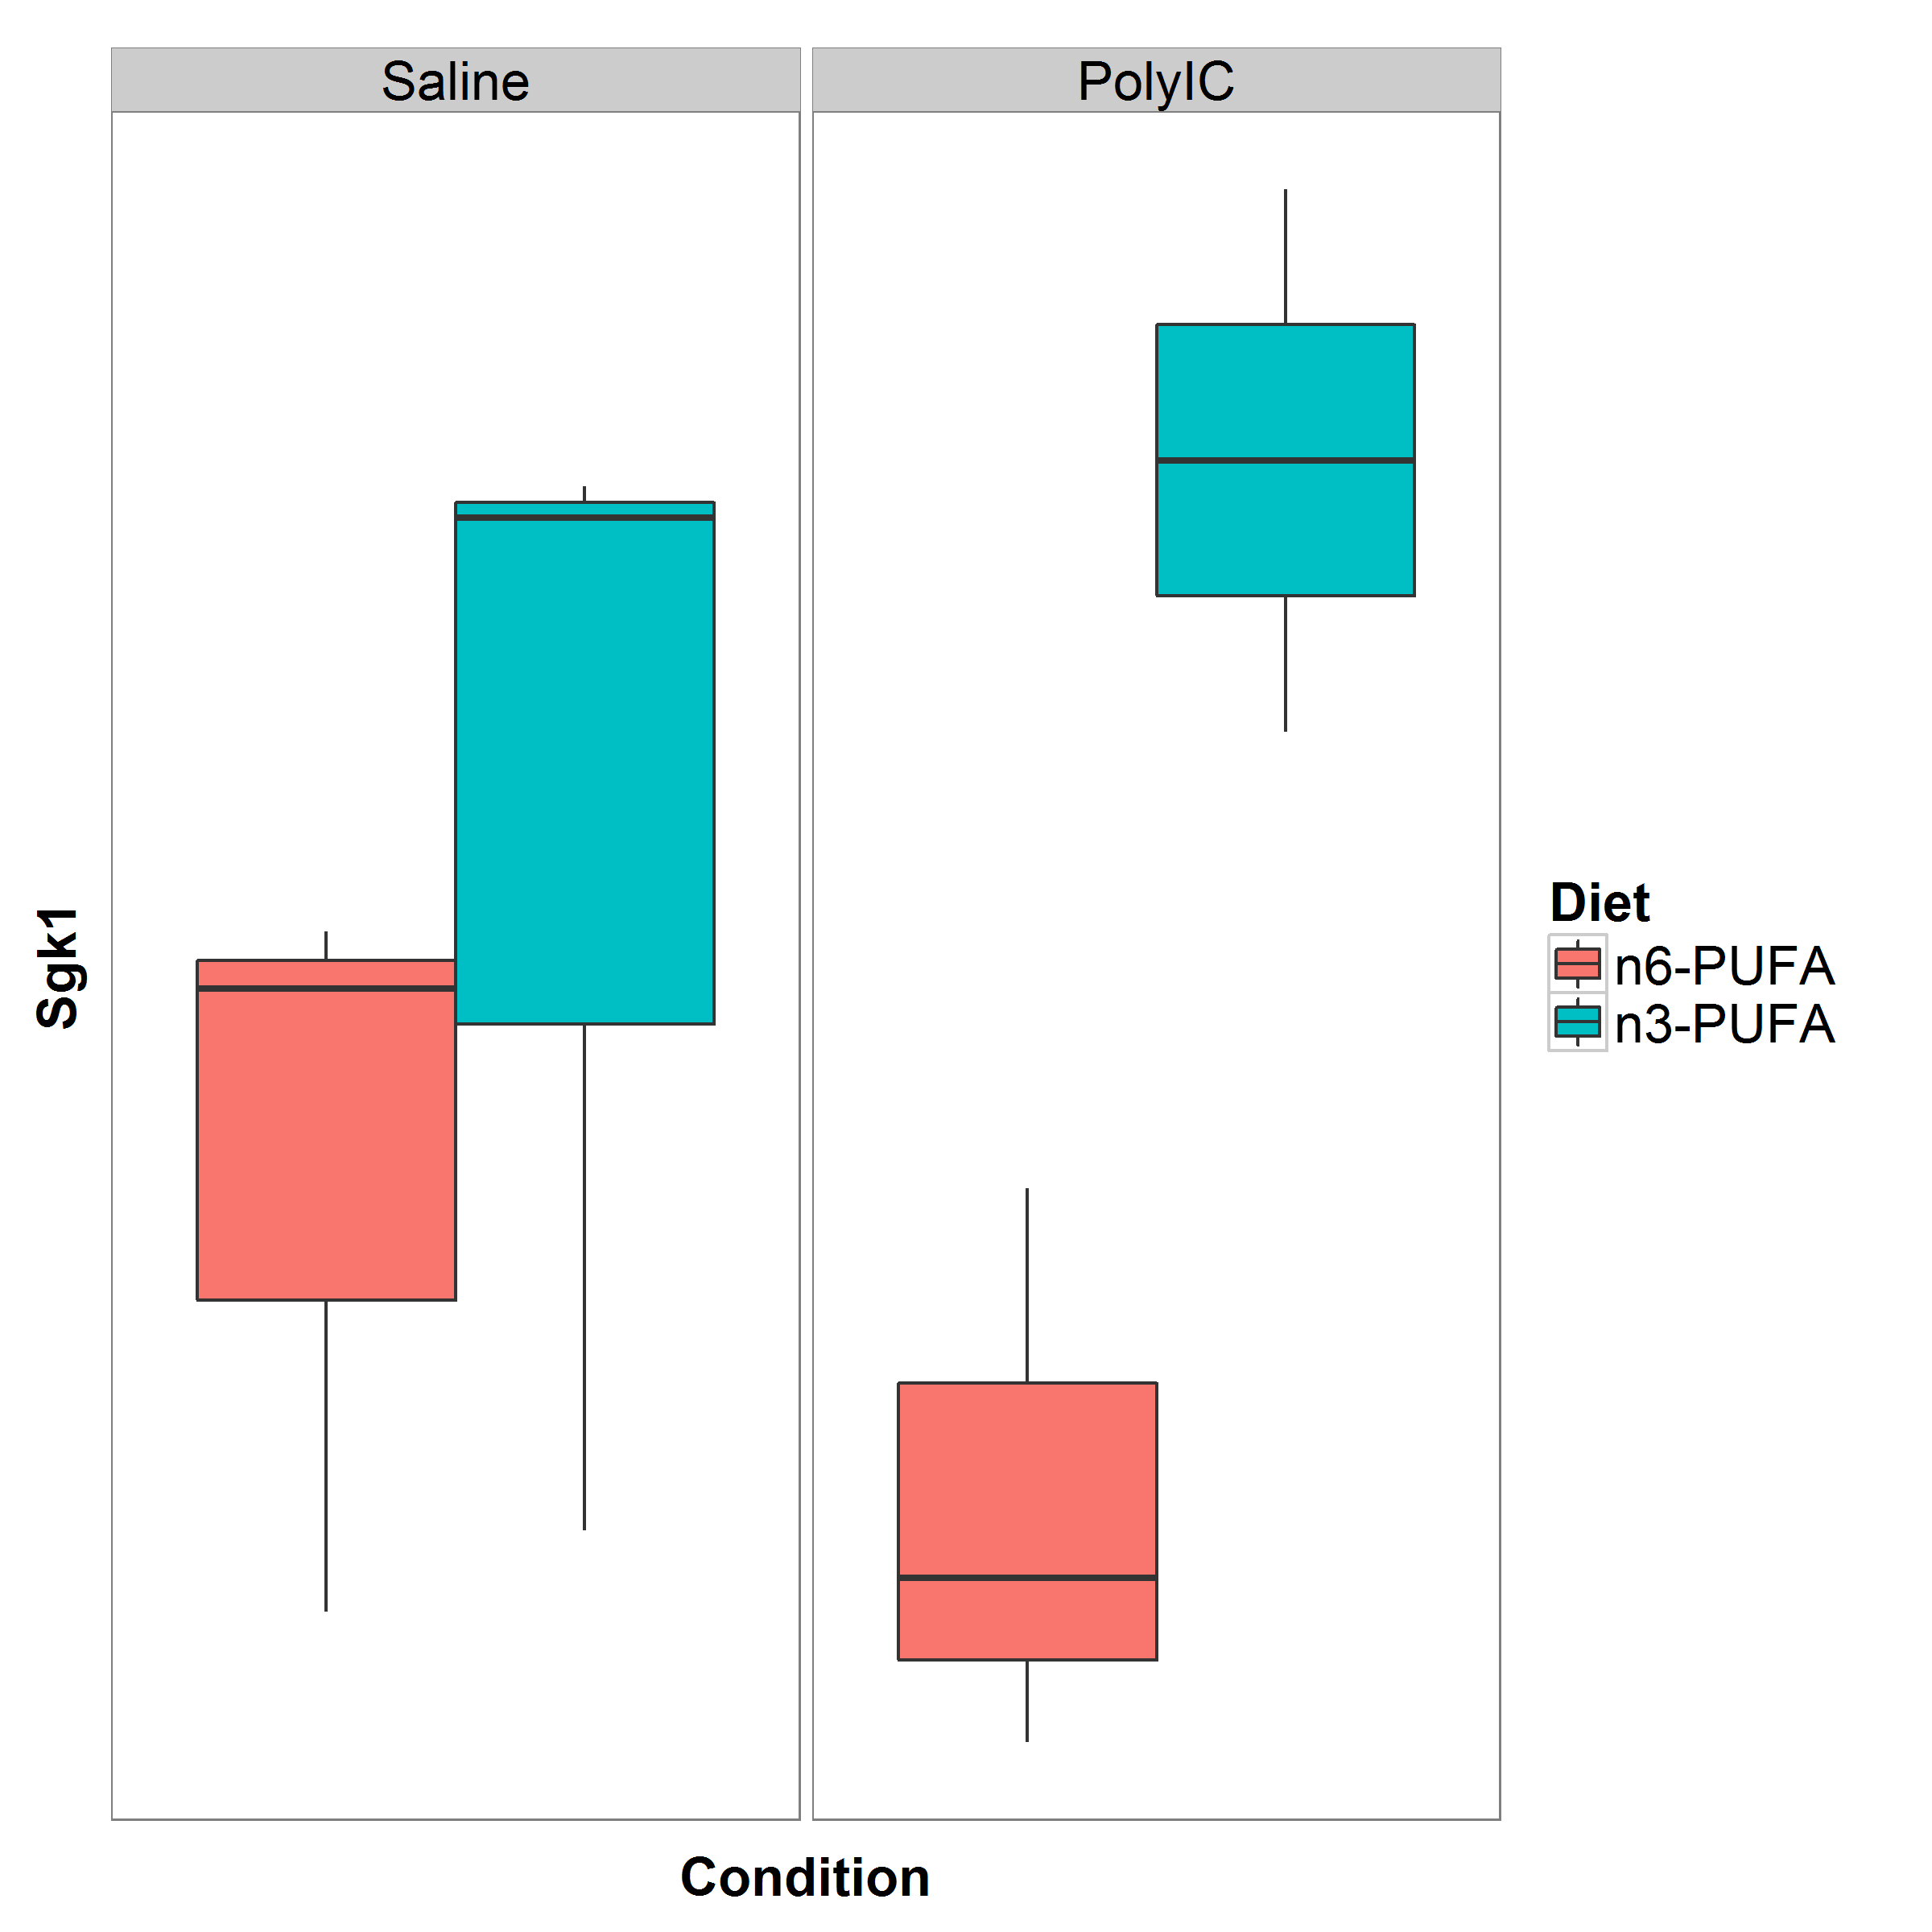
\includegraphics[width=0.6\textwidth]{figure/omega/Sgk1_expression.png}
	\caption[Normalized Expression of \textit{Sgk1}]{
		Normalized Expression of \textit{Sgk1}.
		It was observed that the expression level of \textit{Sgk1} increases after the mice was given a n3-\gls{pufa} rich diet where a significant increase was observed in mice exposed to \gls{polyic}.
	}\label{fig:sgk1Express}
\end{figure}

In our study, it was observed that upon given the n-3 \gls{pufa} rich diet, the \textit{Sgk1} expression in the cerebellum increases (\cref{fig:sgk1Express}).
Although the increase was not significant in the saline mice, a significant up-regulation was observed in the \gls{polyic} exposed mice (\cref{fig:sgk1Express}). 
Additionally, it was also observed that \gls{pi3k} pathways and pathways related to \gls{fgf} receptors and \gls{egf} receptors were significant when studying the effect of n-3 \gls{pufa} rich diet to \gls{polyic} exposed mice.
Upon further investigation, it was found that the \gls{fgf} receptors and \gls{egf} receptors are upstream of the \gls{pi3k}-Akt pathway (\cref{fig:pi3kPathway}) which is responsible for the activation of \textit{Sgk1}.
Although we were unable to provide direct connection between the expression of \textit{Sgk1} and the improve functioning of the \gls{polyic} mice given n-3 \gls{pufa} diet, our results do suggest a possible effect of the n-3 \gls{pufa} rich diet in the expression of genes related to the \gls{pi3k}/Akt pathway and might affect the expression of \textit{Sgk1}.
Further studies are therefore required to understand whether if the change in expression of \textit{Sgk1} can account for the improved functioning of the \gls{polyic} mice. 
A possible design will be to induce the expression of \textit{Sgk1} in \gls{polyic} mice through transfection and examine whether if the \gls{polyic} mice with higher expression of \textit{Sgk1} display a reduction in \glng{scz}-like behaviours.

An important point to note was that previous research of \textit{Sgk1} has been focusing on the hippocampus and not the cerebellum. 
Thus, it is possible that \textit{Sgk1} might have a different function in the cerebellum. 
It is therefore vital for subsequent research to study the effect of \textit{Sgk1} in the cerebellum or for one to study the effect of n-3 \gls{pufa} rich diet on the gene expression in the hippocampus. 

\begin{figure}
	\centering
	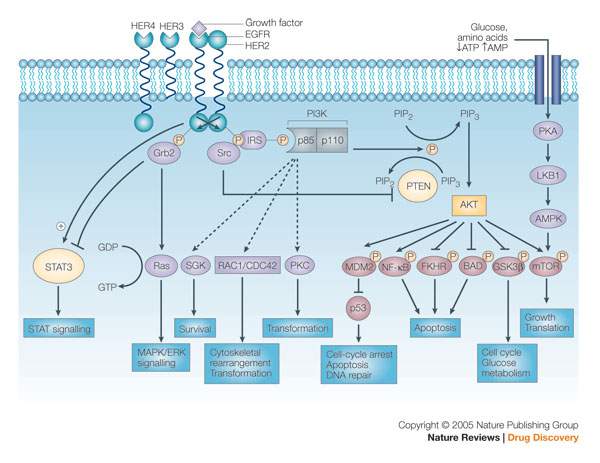
\includegraphics[width=0.6\textwidth]{figure/omega/pi3ksignaling.jpg}
	\caption[Schematic of signalling through the PI3K/AKT pathway]{
		Schematic of signalling through the \gls{pi3k}/AKT pathway.
		It was observed that the growth factors were upstream of the \gls{pi3k}/AKT pathway of which \textit{Sgk1} is one of the member of the pathway.
		Figure adopted from \citet{Hennessy2005} with permission from journal.
	}\label{fig:pi3kPathway}
\end{figure}
\subsection{Functional Annotations}
When examine the expression change in mice exposed to \gls{polyic}, none of the genes were significantly differentiated. 
However, we do observe 12 pathways that contains genes that were more significant than genes not within the pathway (\cref{tab:miaPath}).
Interestingly, of the 12 significant pathways, 5 pathways were related to neuronal functions such as neuroactive ligand-receptor interaction (padj=$1.27\times 10^{-3}$), genes involved in neuronal system (padj=0.00153) and genes involved in transmission across chemical synapses (padj=0.00401).
It has long been developed that the neuronal system and the neurotransmitter regulation plays a critical role in \glng{scz}.
For example, the disruption of the GABAergic and glutamtergic neuronal system might leads to excitation/inhibition imbalance which might ultimately lead to \glng{scz} \citep{Wassef2003}.
Moreover, the alteration in balance betweem excitation and inhibition can distort the connectivity patterns between different brain regions, thus leads to developmental and behavioral deficits \citep{Cline2005}.

Additionally, it was found that the calcium signaling pathway was significant when comparing the effect of \gls{mia}. 
The association of the calcium signaling pathway with \glng{scz} was not a new finding \citep{Lidow2003,Purcell2014,Ripke2014}.
Previous exome sequencing study of \glng{scz} by \citet{Purcell2014} has already report the enrichment of non-synonymous variants within the voltage gate calcium ion channel genes in the \glng{scz} cases and the \gls{pgc} \glng{scz} \gls{GWAS} has also found association between genes encoding the calcium channel subunits with \glng{scz}.
As calcium signaling pathway is the key component of the mechanism responsible for regulating neuronal excitability \citep{Berridge2014}, the disruption of the calcium signaling pathway is likely to have a profound effect on the neural function. 
Together, our results suggest that \gls{mia} might have disrupted the normal functioning of the neural system in the cerebellum, thus lead to schizophrenia-like behaviours in the adult mice yet follow up studies are required to validate our findings.

%TODO quick travel
\glsreset{qqplot}
Moreover, we performed the partitioning of heritability hoping to see whether if the significant pathways have contributes disproportionately to the \gls{SNP} heritability of \glng{scz}.
Interestingly, all 4 significant pathways that were found to be contributing a significantly higher portion to the \gls{SNP} heritability were affected by \gls{mia}.
To assess whether if the significance of these pathways were driven by a small number of very significant genes, we compared the \gls{qqplot} of \glspl{SNP} within the pathway and all the \glspl{SNP} included in the \gls{pgc} \gls{GWAS} (\cref{fig:qqAll}).
It is observed that for most of the pathways, there is a general inflation of summary statistics when compared to the full set, suggest that the significance was not driven by a single significant gene.
However, for the \gls{ecm} related pathway, only a small inflation was observed. 
This is therefore likely that the significance was driven by a small number of significant genes. 

\begin{figure}
	\centering
	\subfloat[\gls{ecm}]{
		\scalebox{.4}{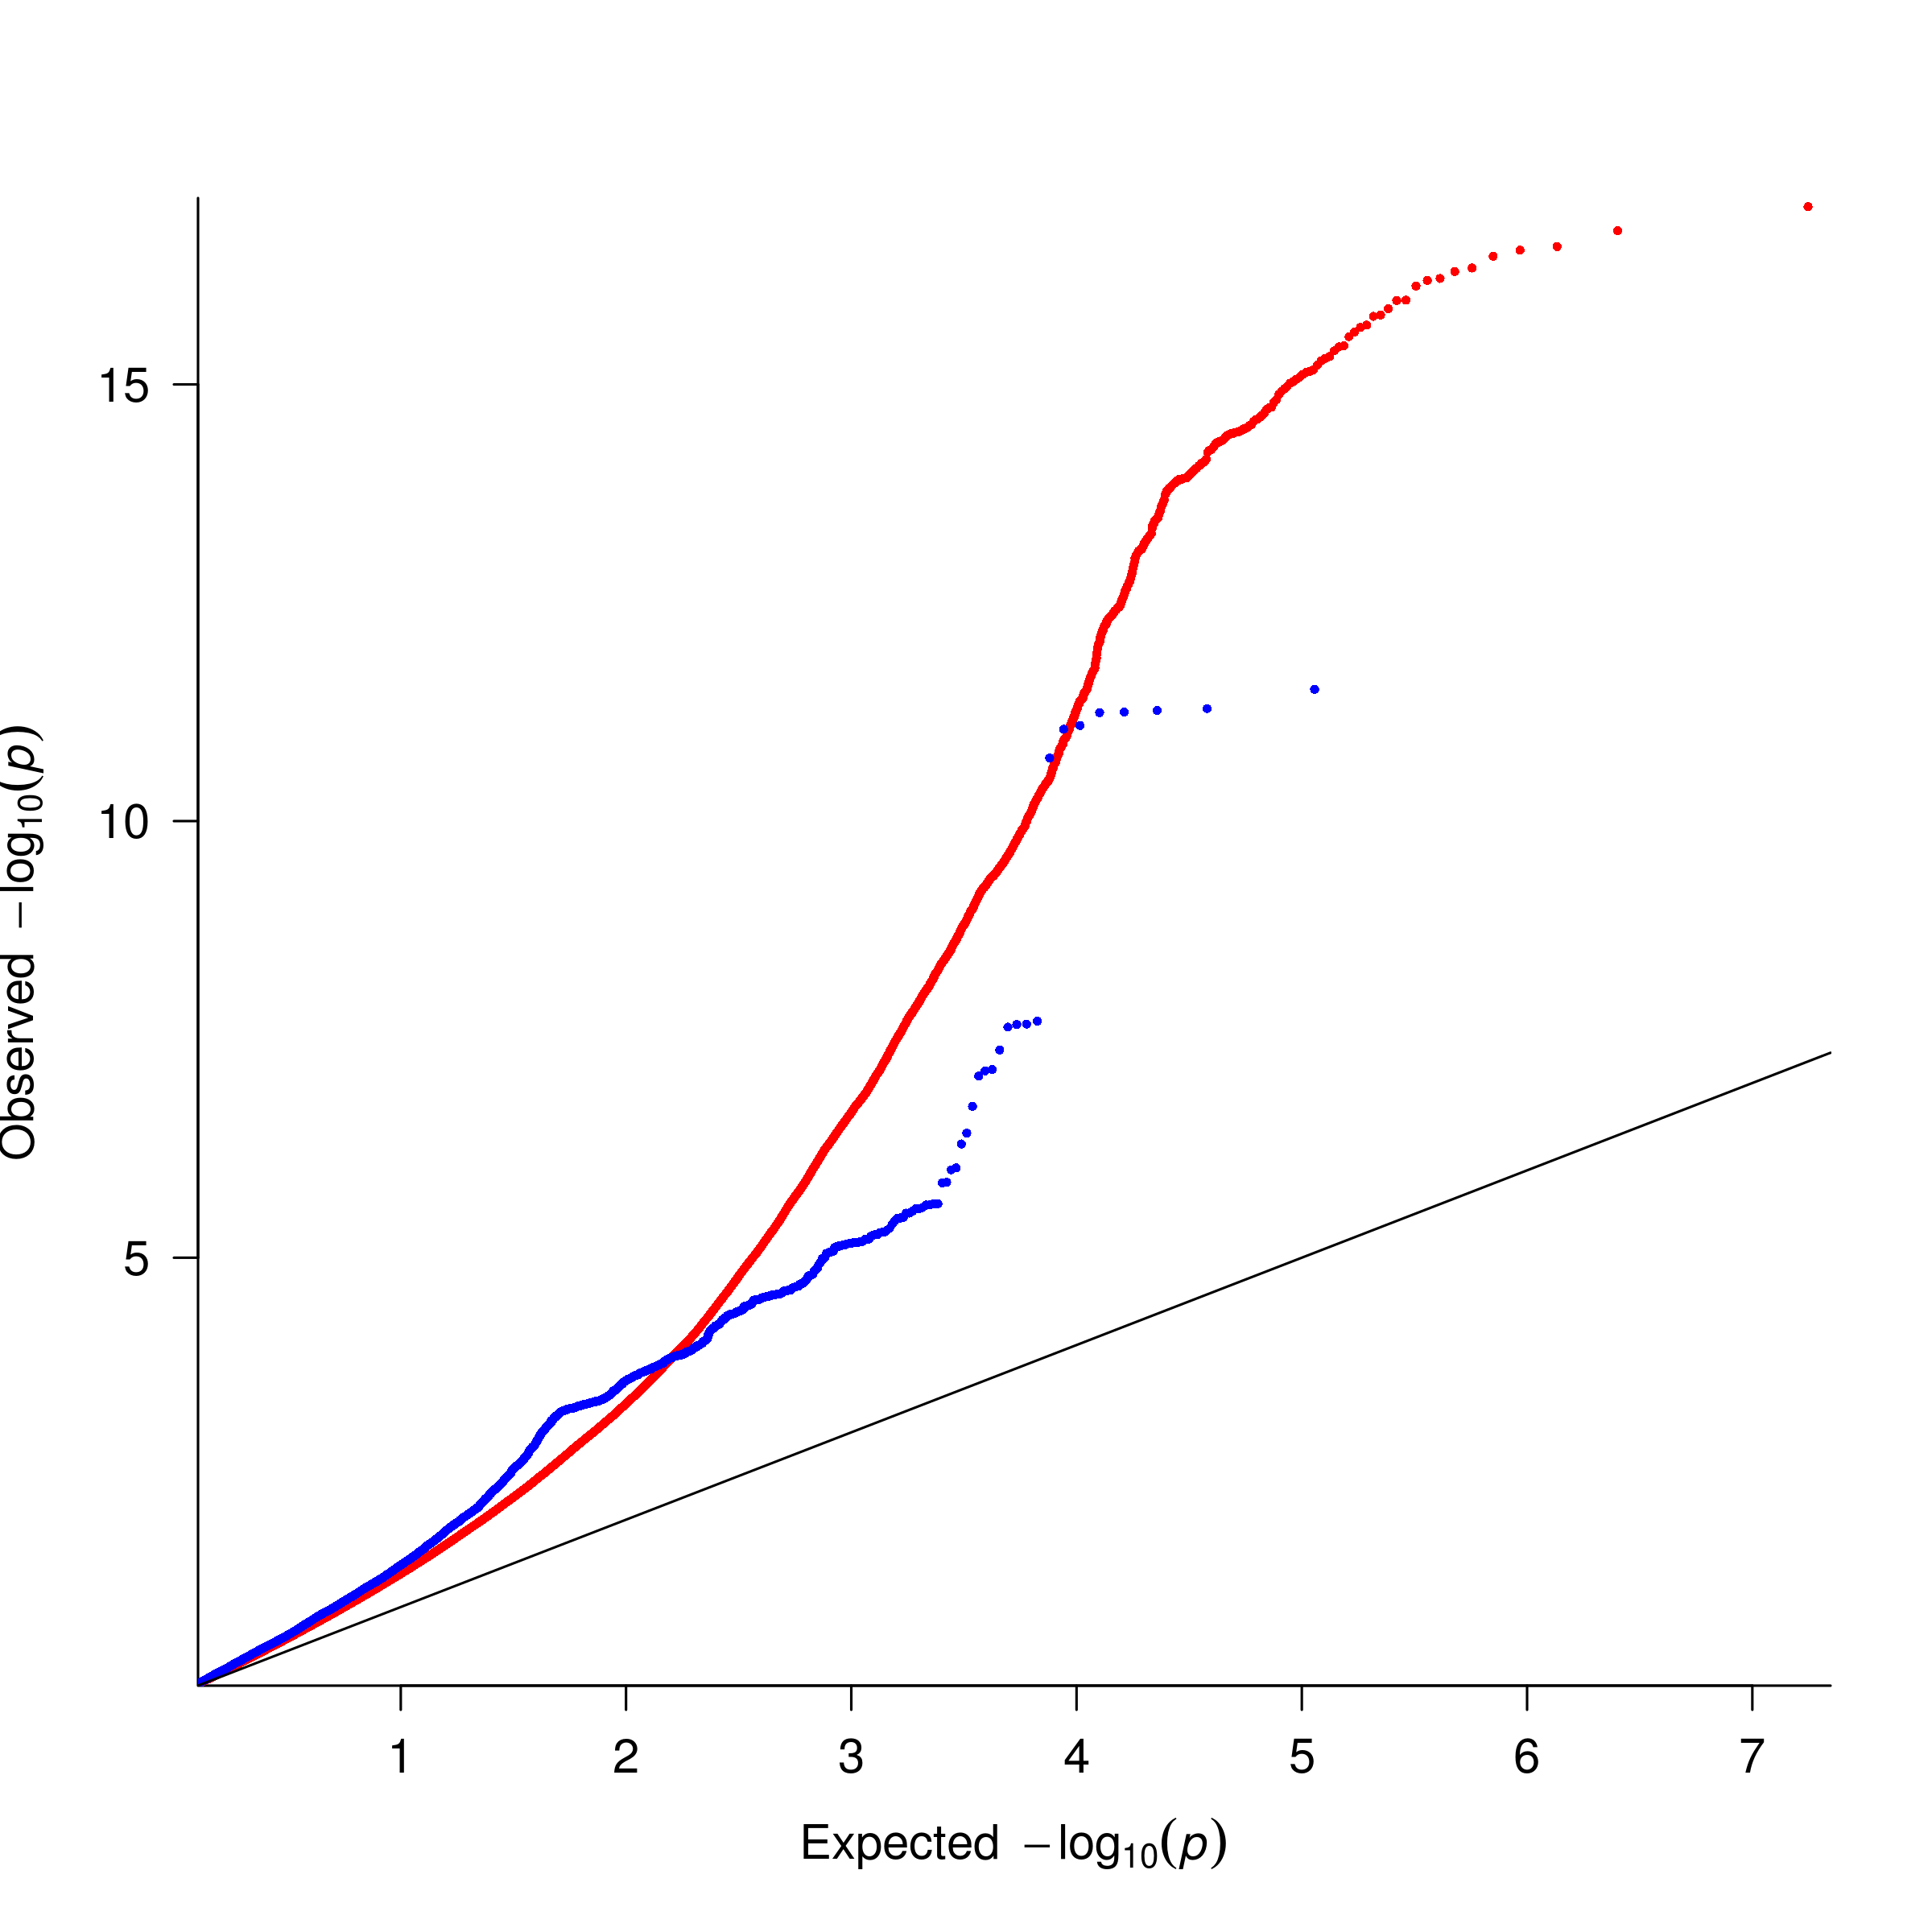
\includegraphics{figure/omega/NABA_CORE_MATRISOME.png}}
		\label{fig:ecm}
	}
	\subfloat[MAPK Signaling]{
		\scalebox{.4}{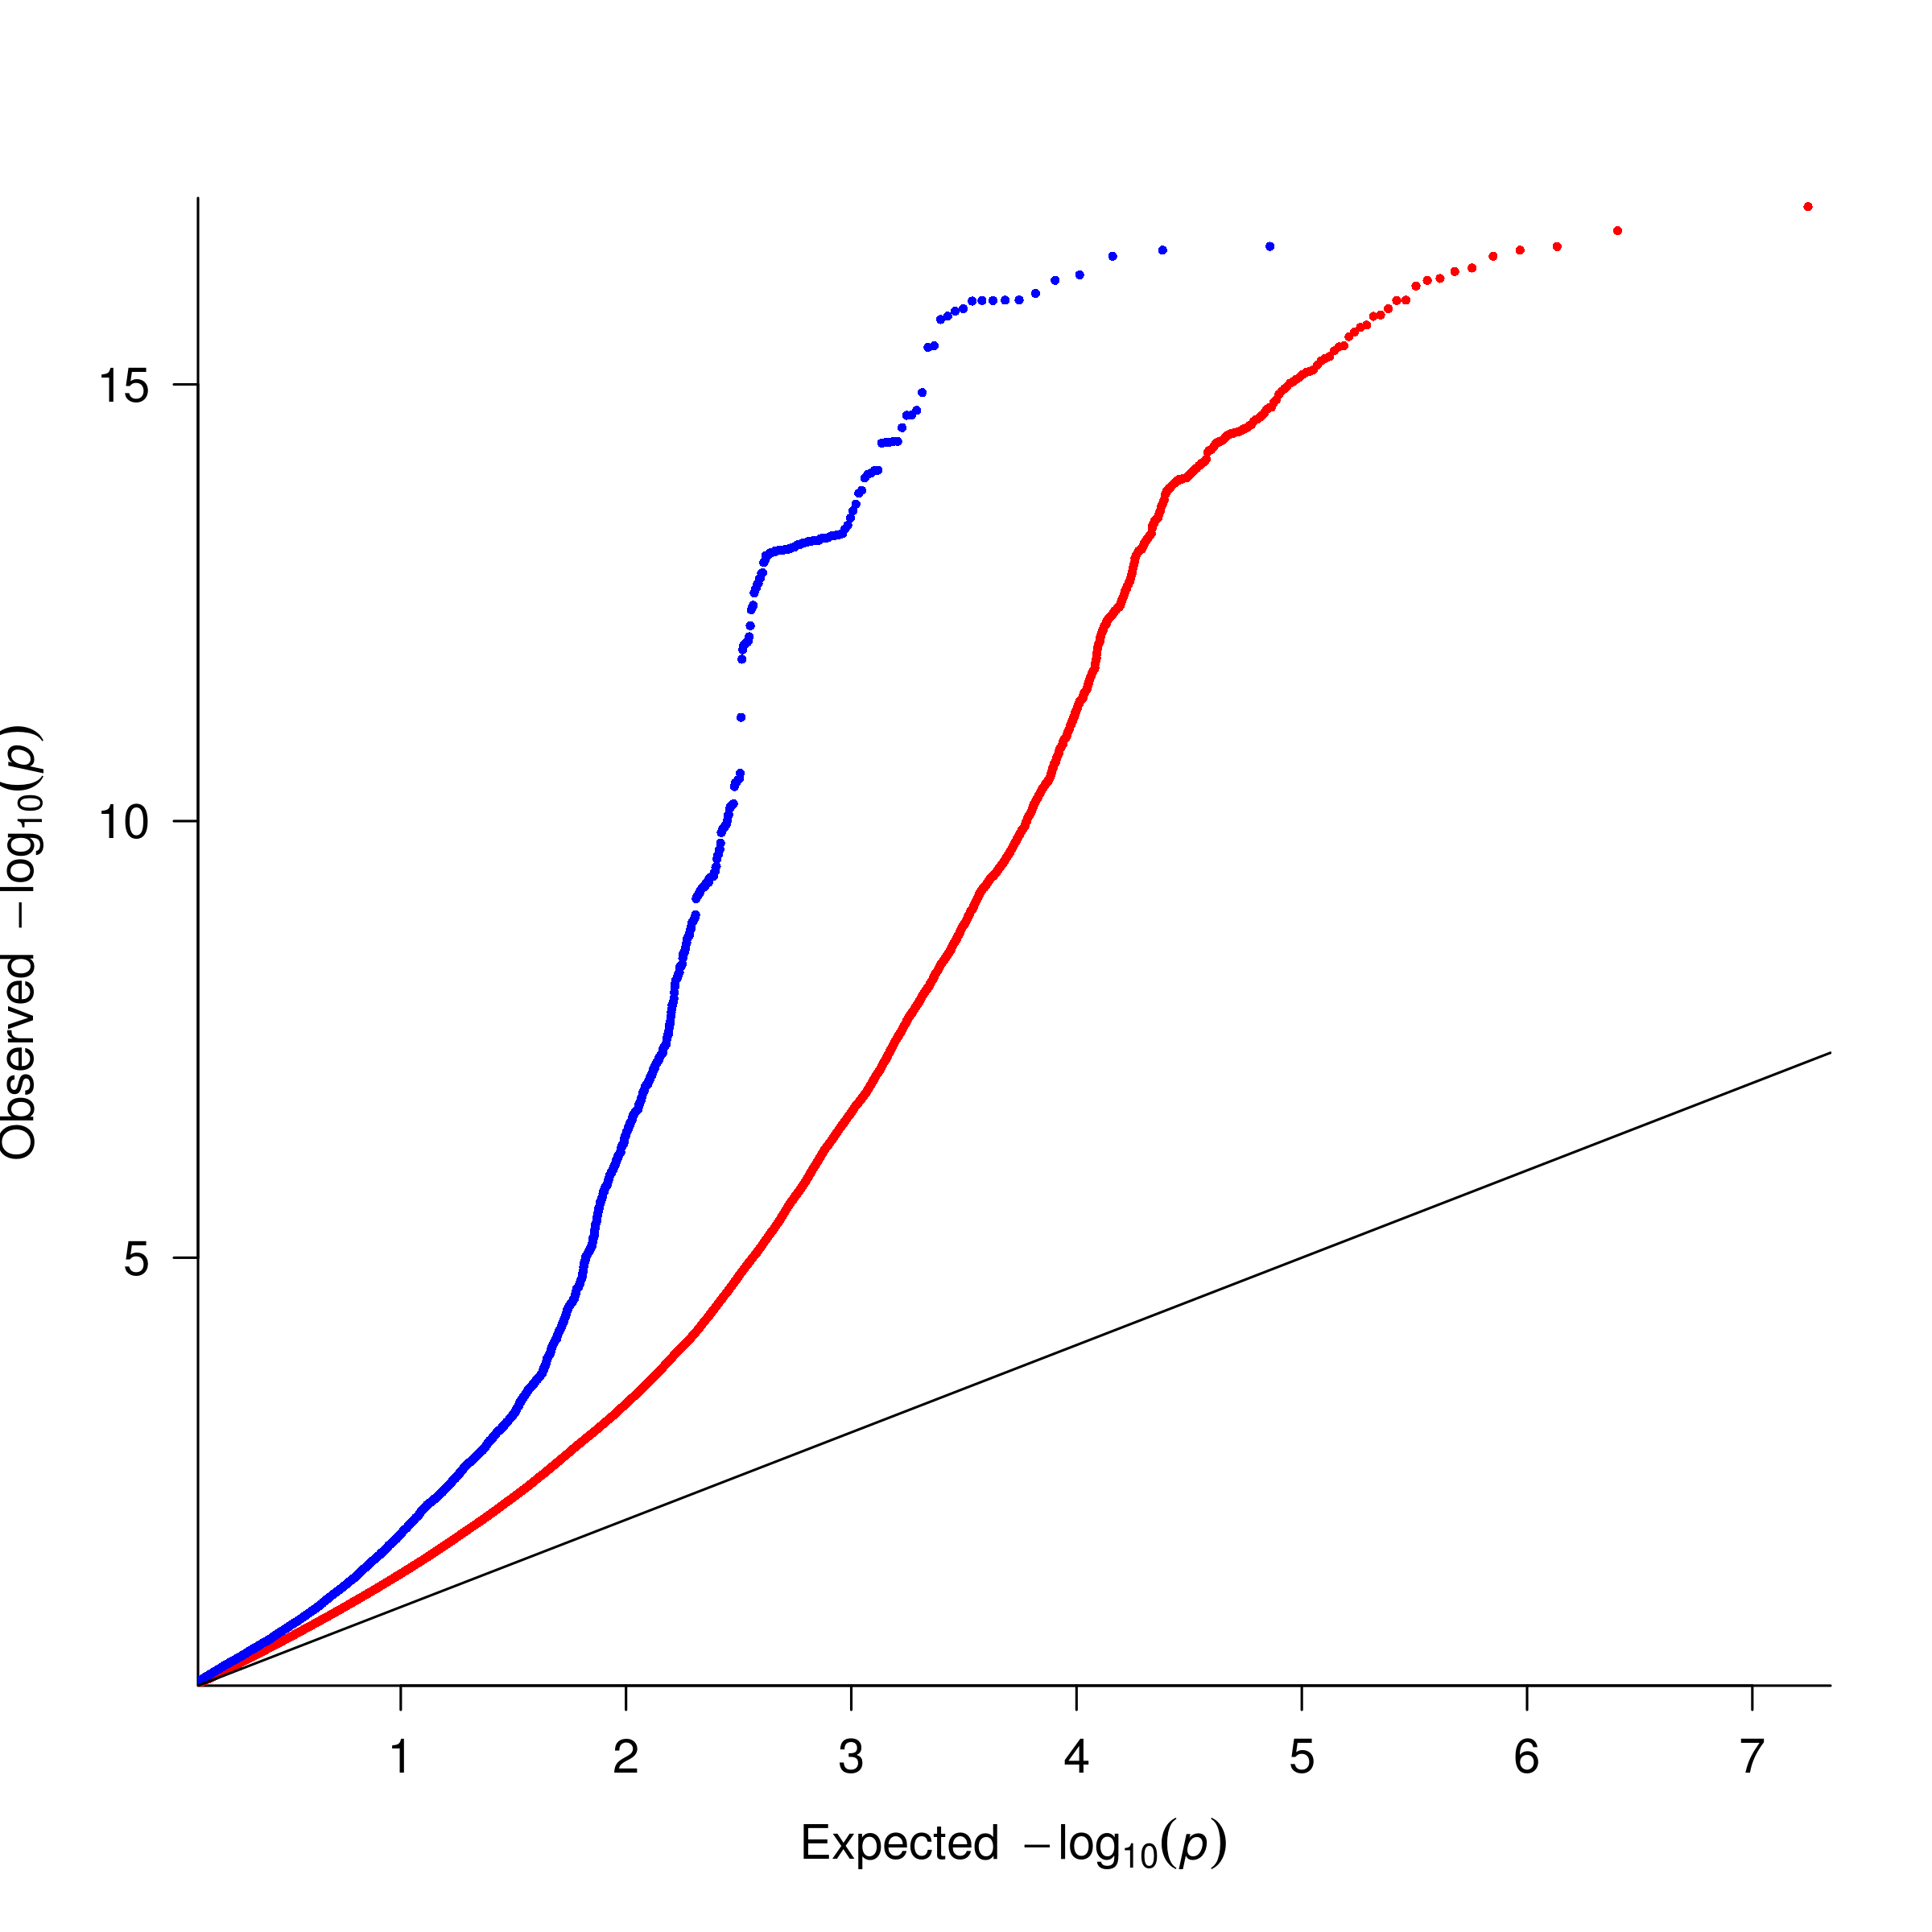
\includegraphics{figure/omega/KEGG_MAPK_SIGNALING_PATHWAY.png}}
		\label{fig:mapk}
	}\\
	\subfloat[Neuronal System]{
		\scalebox{.4}{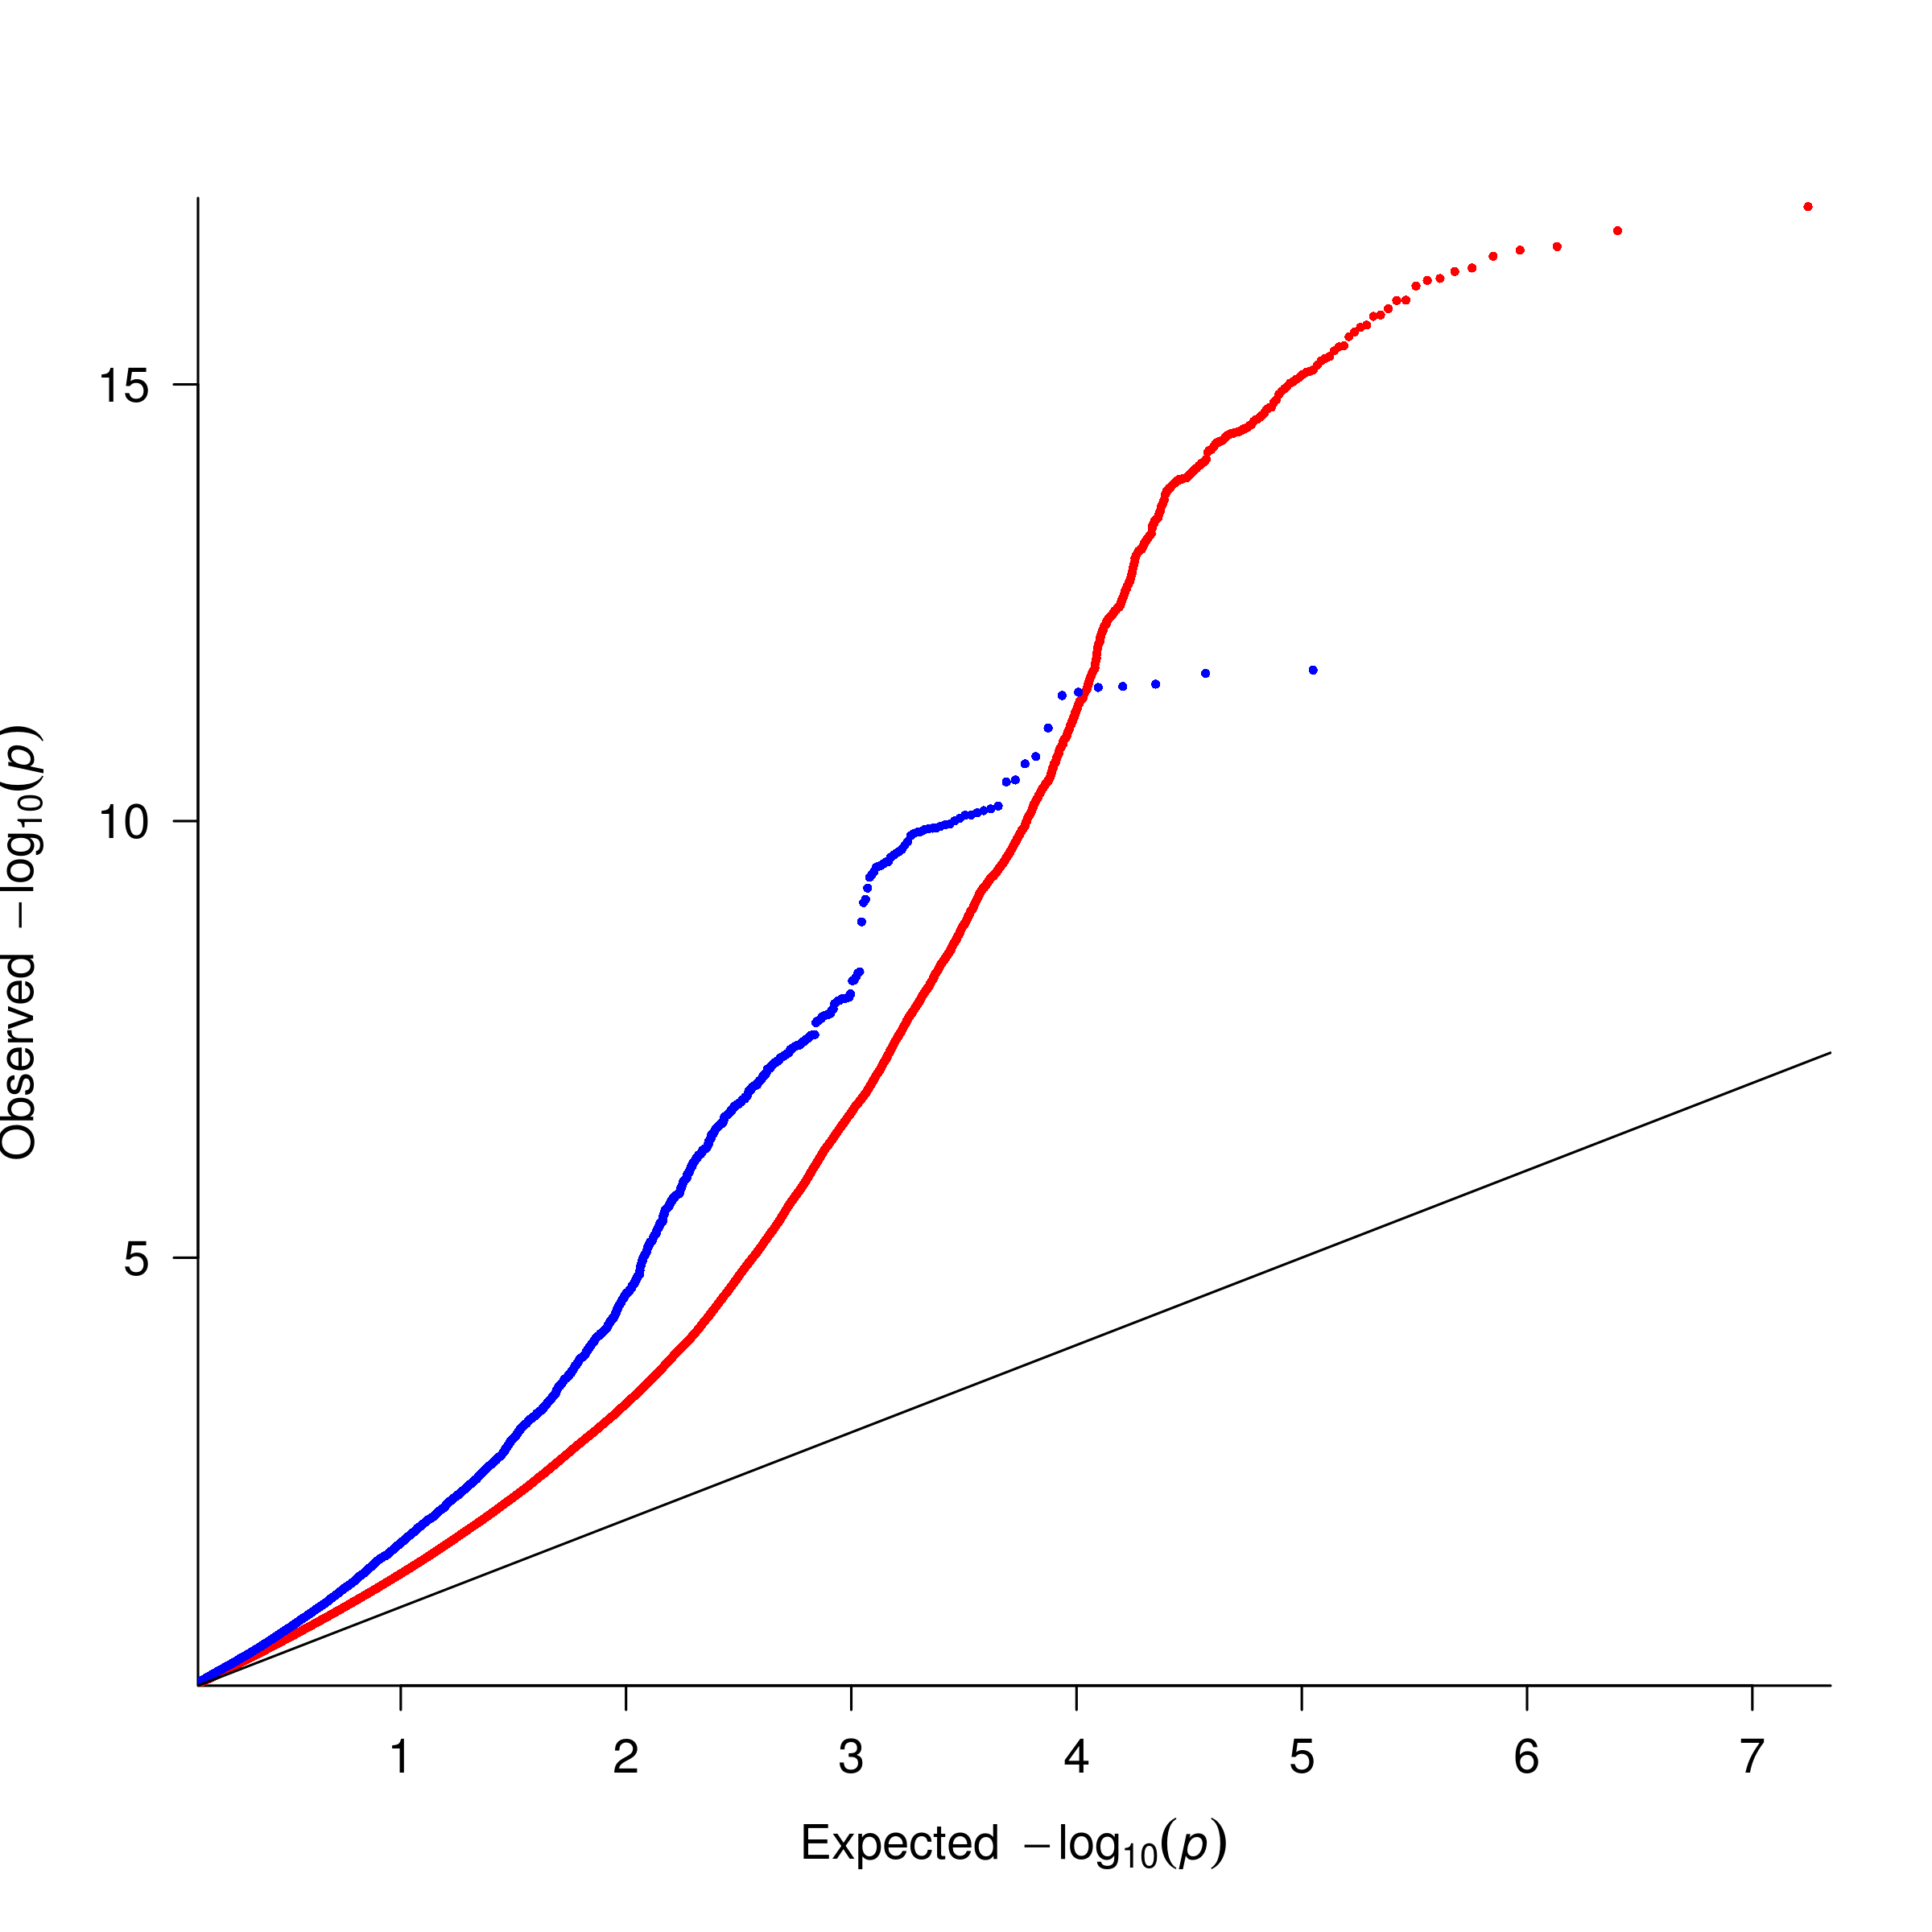
\includegraphics{figure/omega/REACTOME_NEURONAL_SYSTEM.png}}
		\label{fig:neuronal}
	}
	\subfloat[Calcium Signaling]{
		
		\scalebox{.4}{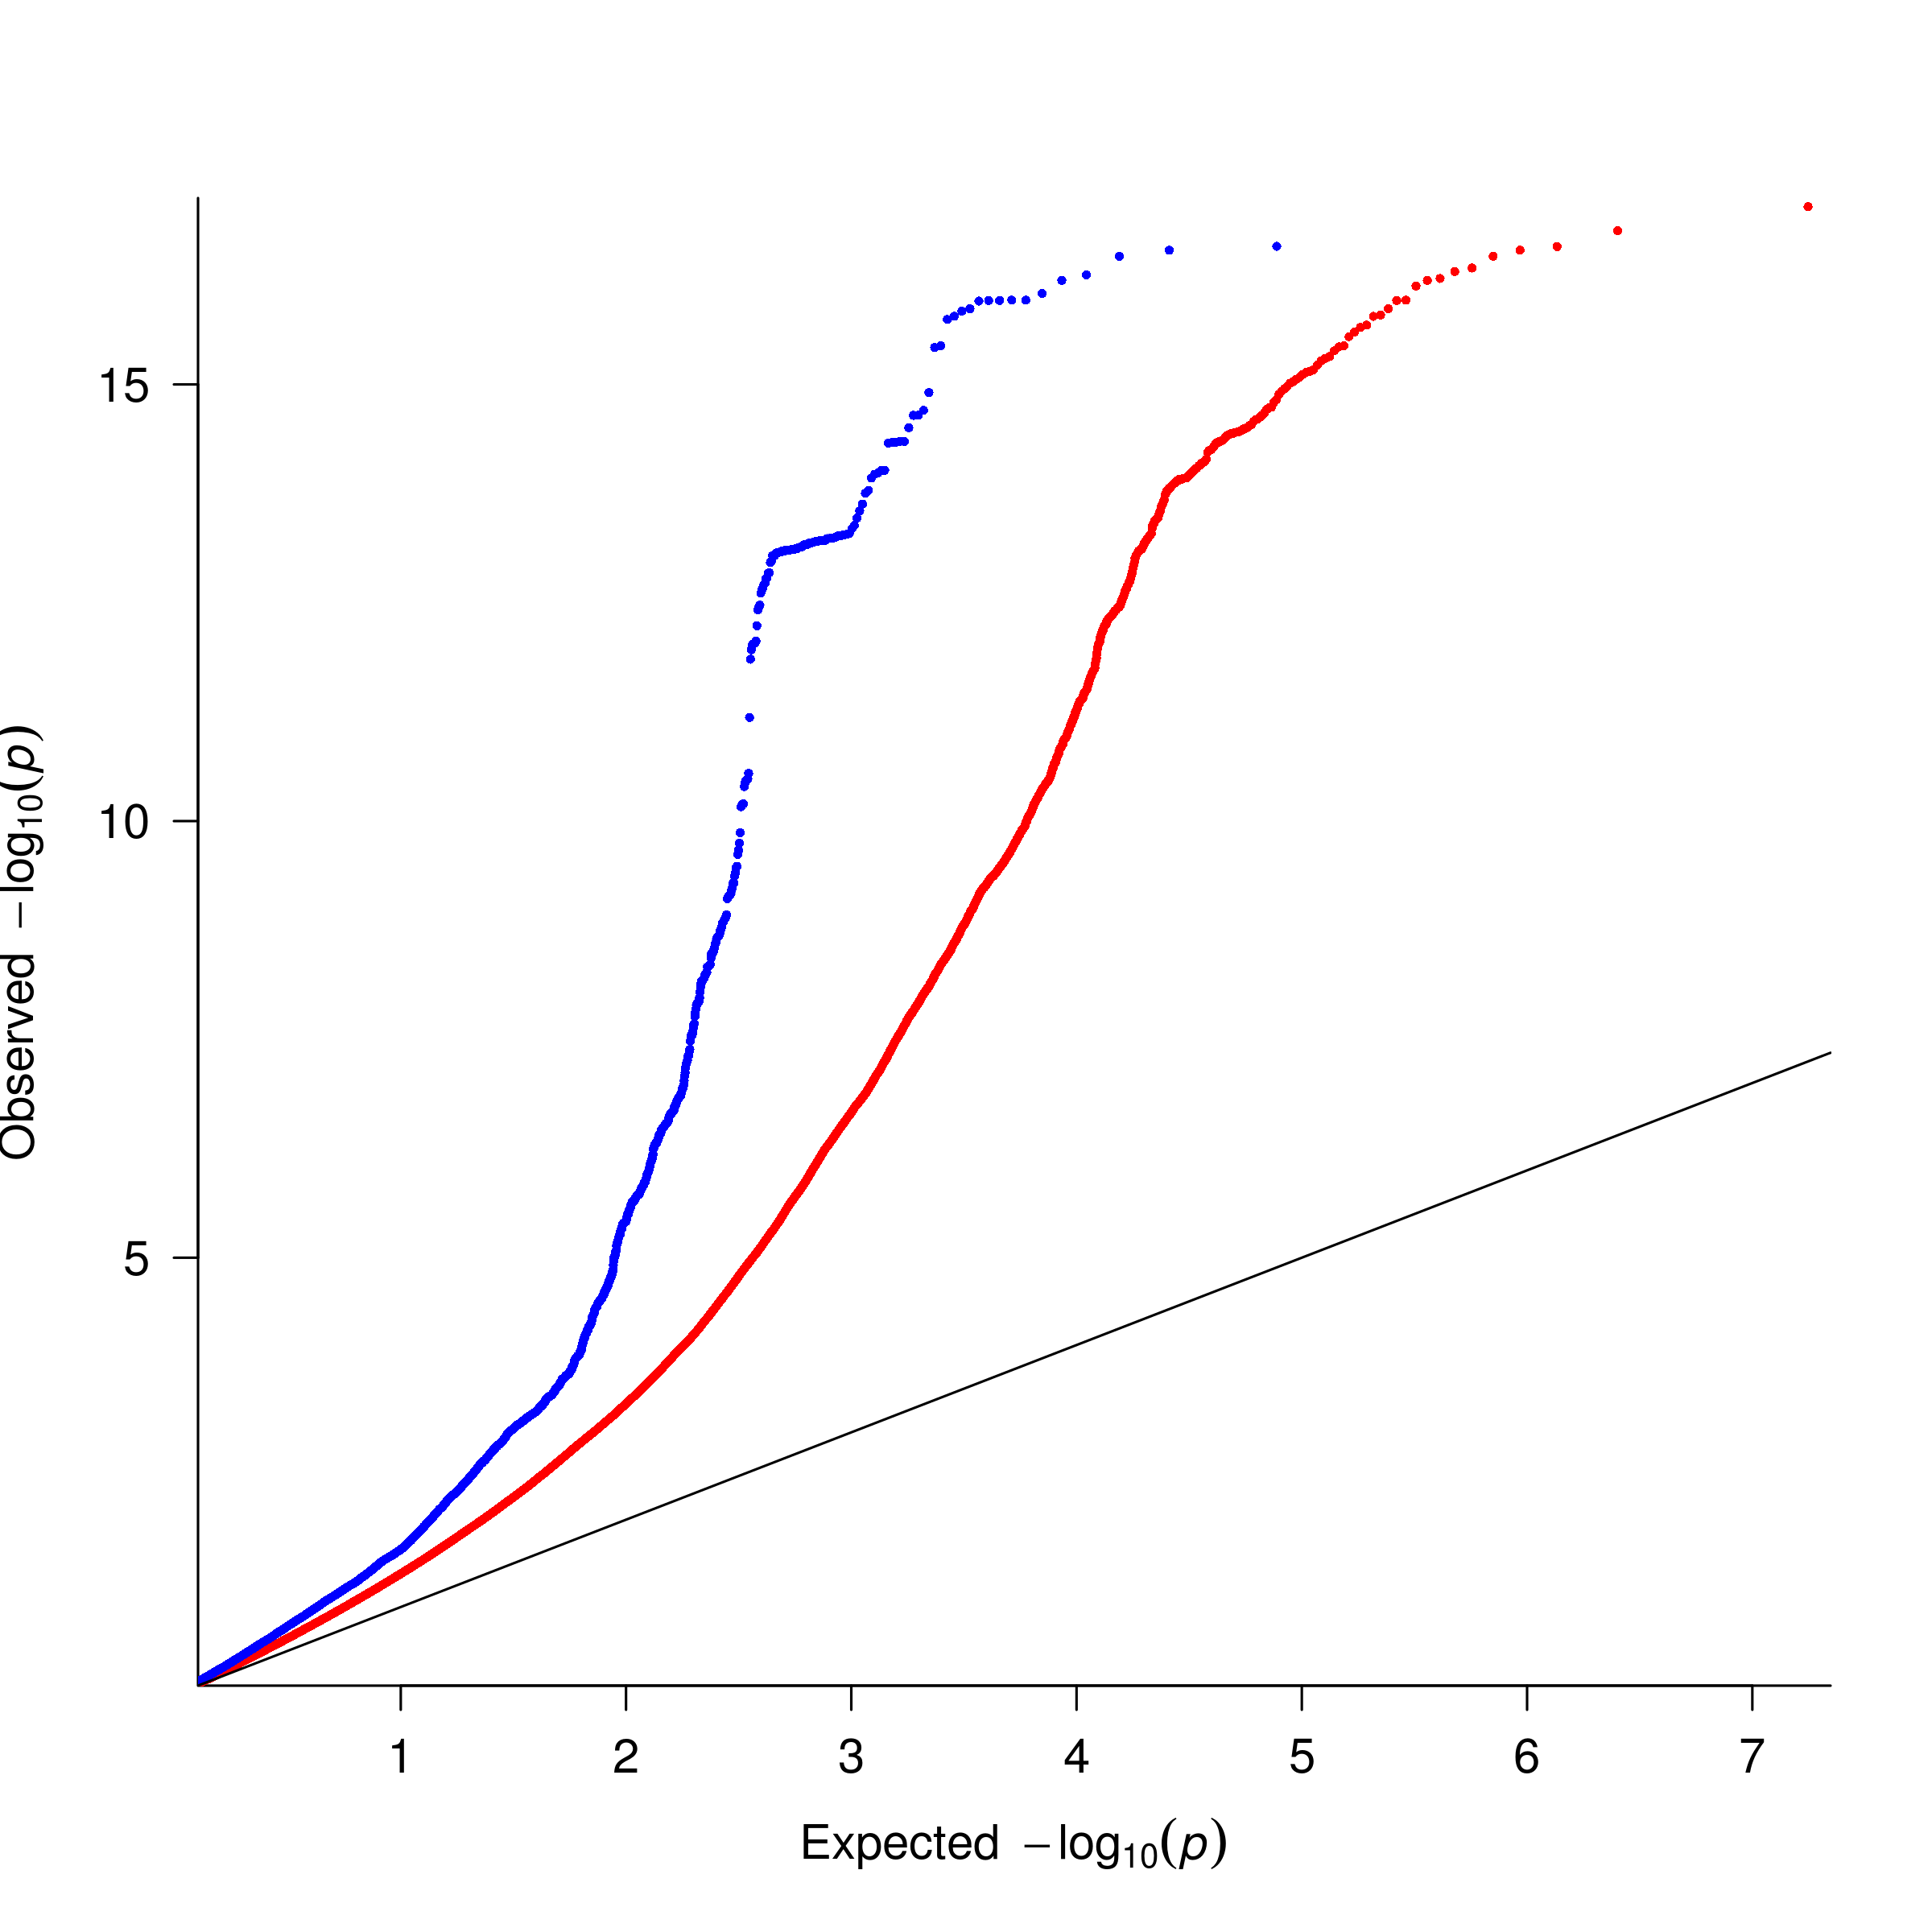
\includegraphics{figure/omega/KEGG_CALCIUM_SIGNALING_PATHWAY.png}}
		\label{fig:calcium}
	}
	\caption[Comparing the QQ plots with PGC SNPs]
	{Comparing the \gls{qqplot} with \gls{pgc} \glspl{SNP}.
		\glspl{SNP} found within the pathways were colored in blue whereas the all the full set of \glspl{SNP} from the \gls{pgc} \gls{GWAS} was coded in red.
		It is observed that for most of the pathways, there is a general inflation of summary statistics when compared to the full set, suggest that the significance was not driven by a single significant gene.
		However, for the \gls{ecm} related pathway, only a small inflation was observed. 
		This is therefore likely that the significance was driven by a small number of significant genes. 
		} 
	\label{fig:qqAll}
\end{figure}

The ``super pathway'' containing all the genes participating in the \gls{mia} related pathways were also found to be significant (\cref{tab:partitioning}) suggest that the differential gene expression in the cerebellum induced by early \gls{mia} events and the genetic variants might act upon similar pathways in the development of \glng{scz}.

Interestingly, among the 4 pathways found to be significantly contributes to the \gls{SNP} heritability, only the pathway related to the assembly of core \gls{ecm} molecules such as the \gls{ecm} glycoproteins, were also found to be significantly affected by the n-3 \gls{pufa} rich diet in the \gls{polyic} exposed mouse. 
Although the \gls{qqplot} suggest that a small number of genes might have driven the significance of this pathway, it is nonetheless an interesting candidate.

Emerging evidences suggest that the \gls{ecm} abnormality might be associated with \glng{scz} \citep{Berretta2012}.
The \gls{ecm} glycoprotein Reelin has been reported to have a decreased expression in the cerebellum of \glng{scz} patients \citep{Maloku2010} and were found to be accompanied by decreased expression of glutamic acid decarboxylase 67 \citep{Costa2001}.
Studies also suggested that Reelin might have important role in corticogenesis and synaptic maturation and stabilization \citep{Berretta2012}.
Moreover, another \gls{ecm} molecule, Semaphorin 3A has been reported to be increased in the cerebellum of subjects with \glng{scz} \citep{Eastwood2003}.
The Semaphroin 3A protein was found to regulates axonal guidance and has a critical role in the  regulation of tangential migration of cortical GABAergic interneurons \citep{Zimmer2010}.
It was also reported that the elevated Semaphorin 3A is associated with down-regulation of genes involved in synaptic formation and maintenance \citep{Eastwood2003}.
Together, these evidence suggest that the \gls{ecm} molecules might have critical role in the development of \glng{scz}.

It has been reported that the n-3 \gls{pufa} diet can modulate the \gls{mmp} \citep{Derosa2009,Kavazos2015} which can regulates the \gls{ecm} composition \citep{Stamenkovic2003}.
Therefore it is possible that the n-3 \gls{pufa} diet has exerted its effect to the \gls{ecm} through \gls{mmp}.
However, from the \gls{qqplot}, it was noted that only a modest inflation was observed (\cref{fig:ecm}).
This suggest that the significance of the \gls{ecm} pathway might have been driven by a small number of significant genes.
Due to difficulties in delineating the individual \glspl{SNP} effect, it is difficult for us to pin-point the ``driver'' genes of this pathway.
Moreover, none of the \gls{ecm} genes were found to be differentially expressed in either of our condition, therefore we urge that further studies are required to understand how the n-3 \gls{pufa} direct interacts with the \gls{ecm} or the \gls{ecm} related genes and the effect of such interaction in \gls{mia} exposed individuals.

Finally, it is important to note that the current study serves only as a hypothesis generation study and the sample size was modest. 
We therefore like to use the current results to provide an estimation of sample size required for a replication study.
By using Scotty \citep{Busby2013}, we have estimated that the replication study should contain at least 10 samples for each group in order for us to detect at least 80\% of genes has at least 80\% of the maximum power. 
We have also demonstrated that the batch effect can have a big impact to the association (\cref{fig:batchLRT}), therefore one should always control for the batch effect whenever possible.
Given the current resources, one of the preferred design for the follow up study are given in \cref{tab:bestdesign}.

\subsection{Limitations}
We first acknowledge that the sample size of the current study is small and are underpowered.
This is reflected in the \glspl{qqplot} (\cref{fig:waldQQ}) where the observed p-values were generally smaller than would have expected.
A better study design will include more samples yet we were limited by our budget.
However, the importance of a pilot study is to identify potential targets for replications, hypothesis generation or to provide guidance for follow up studies. 
In this study, we have identified \textit{Sgk1} as an interesting candidate gene that might have an important role in the effect of n-3 \gls{pufa} in \gls{polyic} exposed individuals.
Our results provide support for a possible converging functional effect of differential expression induced by early \gls{mia} and genetic variations observed in \glng{scz}.
These provide interesting candidates for follow studies and we were able to estimate and design a better replication study based on the current data. 
Therefore we argue that as a hypothesis generation study, our study is successful.

Second, we examined only the male brains in the current study. 
The decision to direct experimental resources to males was made because there is evidence that the male fetus is more vulnerable to environmental exposures such as inflammation in prenatal life \citep{Bergeron2013,Lein2007}. 
We acknowledge that an interesting follow up study would be to investigate the gender difference in response to \gls{mia} and dietary change.

Third, although RNA Sequencing was performed, we did not performed any analysis on possible alternative splicing events or denovo transcript assembly.
The reason behind such decision is that our sample size is simply too small.
Without sufficient information, denovo transcript assembly can return noisy results.
On the other hand, in order to investigate possible alternative splicing events, we would need to perform the analysis on transcript level instead of gene level. 
This increase the possible candidates from 47,400 genes to 114,083 transcripts.
Combining with the difficulties of the quantification of different isoforms, a much larger power is required for the alternative splicing analysis. 
On top of that, the functional annotation of transcripts is another difficult aspect to tackle.
While there are a lot of information for the annotation of genes, information on functional difference between isoforms of the same gene are generally lacking. 
The lack of annotation leads to difficulties in making sense of the data. 
Thus although we acknowledge the possible importance of alternative splicing and denovo transcripts, we did not perform any alternative splicing analysis or denovo transcripts assembly.
Nonetheless, the use of RNA Sequencing allow us to easily perform these experiments once sufficient samples are obtained.

Forth, it is important to note that a high RNA expression level does not guarantee a high protein concentration \citep{Vogel2012}.
Post transcriptional, translational and degradation regulation can all affect the rates of protein production and turnover, therefore contributes to the determination of protein concentrations, at least as much as transcription itself \citep{Vogel2012}.
The RNA Sequencing thus only provide an approximation to the concentration of a particular protein in the samples.
However, we do argues that RNA Sequencing can help to identify potential targets for protein assays where detail analysis can be performed on the protein level.

Finally, at the time of this thesis, we have yet completed any \gls{rtpcr} or any functional studies to validate our findings.
One of the most vital steps after any RNA Sequencing results is to validate the differential expression findings using the \gls{rtpcr}.
Ideally, not only should one perform the \gls{rtpcr} on the sequenced samples, one should also perform the \gls{rtpcr} on an independent set of samples. 
Moreover, the RNA Sequencing only helps to identify possible candidates that were ``associated'' with a particular trait.
It does not provide any causal linkage between the phenotype and the differential expression.
If one would like to establish a direct linkage between the phenotype and the expression of a gene, one will need to carry out functional studies such as knock-in knock-out mouse design.
For example, in order to understand the functional impact of the differential expression of \textit{Sgk1}, one might try to examine whether if the pure up-regulation of \textit{Sgk1} through transfection can reduce the \glng{scz}-like behavior in \gls{polyic} exposed mice.

Currently, we are planning to perform the \gls{rtpcr} on \textit{Sgk1} on all available samples. 
Shall the results be validated, we can then perform subsequent functional studies. 

\newpage
\section{Supplementary}
% Table generated by Excel2LaTeX from sheet 'Sheet1'
\begin{center}
	\begin{longtable}[H]{rrrrrr}
			\toprule
			Litter & Condition & Diet  & Cage  & Batch & Lane \\
			\midrule
			\endhead
			\hline
			\multicolumn{6}{c}{Continued}\\
			\bottomrule
			\endfoot
			\bottomrule
			\endlastfoot
			    1     & PolyIC & n-3 PUFA & 1     & 1     & 1 \\
			    1     & PolyIC & n-6 PUFA & 2     & 5     & 1 \\
			    2     & PolyIC & n-3 PUFA & 3     & 4     & 2 \\
			    2     & PolyIC & n-6 PUFA & 4     & 3     & 3 \\
			    3     & PolyIC & n-3 PUFA & 5     & 2     & 4 \\
			    3     & PolyIC & n-6 PUFA & 6     & 1     & 1 \\
			    4     & PolyIC & n-3 PUFA & 7     & 5     & 1 \\
			    4     & PolyIC & n-6 PUFA & 8     & 4     & 2 \\
			    5     & PolyIC & n-3 PUFA & 9     & 3     & 3 \\
			    5     & PolyIC & n-6 PUFA & 10    & 2     & 4 \\
			    6     & PolyIC & n-3 PUFA & 1     & 2     & 1 \\
			    6     & PolyIC & n-6 PUFA & 2     & 1     & 2 \\
			    7     & PolyIC & n-3 PUFA & 3     & 5     & 2 \\
			    7     & PolyIC & n-6 PUFA & 4     & 4     & 3 \\
			    8     & PolyIC & n-3 PUFA & 5     & 3     & 4 \\
			    8     & PolyIC & n-6 PUFA & 6     & 2     & 1 \\
			    9     & PolyIC & n-3 PUFA & 7     & 1     & 2 \\
			    9     & PolyIC & n-6 PUFA & 8     & 5     & 2 \\
			    10    & PolyIC & n-3 PUFA & 9     & 4     & 3 \\
			    10    & PolyIC & n-6 PUFA & 10    & 3     & 4 \\
			    11    & Saline & n-3 PUFA & 1     & 3     & 1 \\
			    11    & Saline & n-6 PUFA & 2     & 2     & 2 \\
			    12    & Saline & n-3 PUFA & 3     & 1     & 3 \\
			    12    & Saline & n-6 PUFA & 4     & 5     & 3 \\
			    13    & Saline & n-3 PUFA & 5     & 4     & 4 \\
			    13    & Saline & n-6 PUFA & 6     & 3     & 1 \\
			    14    & Saline & n-3 PUFA & 7     & 2     & 2 \\
			    14    & Saline & n-6 PUFA & 8     & 1     & 3 \\
			    15    & Saline & n-3 PUFA & 9     & 5     & 3 \\
			    15    & Saline & n-6 PUFA & 10    & 4     & 4 \\
			    16    & Saline & n-3 PUFA & 1     & 4     & 1 \\
			    16    & Saline & n-6 PUFA & 2     & 3     & 2 \\
			    17    & Saline & n-3 PUFA & 3     & 2     & 3 \\
			    17    & Saline & n-6 PUFA & 4     & 1     & 4 \\
			    18    & Saline & n-3 PUFA & 5     & 5     & 4 \\
			    18    & Saline & n-6 PUFA & 6     & 4     & 1 \\
			    19    & Saline & n-3 PUFA & 7     & 3     & 2 \\
			    19    & Saline & n-6 PUFA & 8     & 2     & 3 \\
			    20    & Saline & n-3 PUFA & 9     & 1     & 4 \\
			    20    & Saline & n-6 PUFA & 10    & 5     & 4 \\
			\bottomrule
		\caption[Design for Follow Up Study]{
			Design for follow up study.
			This design will allow one to balanced out litter effect, cage effect, batch effect and lane effects such that the confounding effects were minimized.
			One can also include the \gls{ercc} spike in control to serves as an internal standard for additional level of control \citep{Jiang2011a}.
			}
		\label{tab:bestdesign}%
	\end{longtable}%ssss
\end{center}
% End up it is very easy, all you have to do is to first sort the table with the previous condition then e.g. Cage, then repeat the number of condition e.g. 1,2,1,2,1,2 until the end. Keep doing that and you will have a best mixed model